%% ----------------------------------------------------------------------------
% BIWI SA/MA thesis template
%
% Created 09/29/2006 by Andreas Ess
% Extended 13/02/2009 by Jan Lesniak - jlesniak@vision.ee.ethz.ch
% Updated 16/03/2023 by Danda Pani Paudel - paudel@vision.ee.ethz.ch
%% ----------------------------------------------------------------------------
\documentclass[pdftex,10pt,openright,headsepline,twoside]{book}
\usepackage[margin=1in,headheight=13.6pt]{geometry}

\usepackage{paralist}		% List environment
\usepackage{color}		% For colored text
\usepackage{times}
\usepackage{amsfonts}		% Additional math fonts
\usepackage{amsmath}		% Math symbols
\usepackage{latexsym}
\usepackage{graphicx}		% For including images
\usepackage{listings}		% If listings are needed
\usepackage{packages/mydefs}		% Some of our own definitions
% \usepackage{wrapfig}		% To wrap images
% \usepackage{algorithmic}	% Nice algorithm environment
% \usepackage{algorithm}
\usepackage{fancyhdr}		% Produce the nice header
%\usepackage{fullpage} % Use the full page

% ========= CHANGES ==================================
\usepackage[english]{babel}
\usepackage[utf8]{inputenc}
\usepackage[T1]{fontenc}
\usepackage[backend=biber, bibencoding=utf8]{biblatex}
\bibliography{bib/references}
\usepackage{csquotes}
\usepackage[hidelinks=true]{hyperref}
\usepackage{bm}
\usepackage{blindtext}
\usepackage[font=small, labelfont=bf]{caption}
\usepackage{tabularx}
\usepackage{algorithm}
\usepackage{algpseudocode}
\usepackage{tikz}
\DeclareMathOperator*{\argmax}{argmax}
\DeclareMathOperator*{\argmin}{argmin}
\lstset{language=Python,keywordstyle={\color{blue}}}
\definecolor{maroon}{cmyk}{0, 0.87, 0.68, 0.32}
\definecolor{halfgray}{gray}{0.55}
\definecolor{ipython_frame}{RGB}{207, 207, 207}
\definecolor{ipython_bg}{RGB}{247, 247, 247}
\definecolor{ipython_red}{RGB}{186, 33, 33}
\definecolor{ipython_green}{RGB}{0, 128, 0}
\definecolor{ipython_cyan}{RGB}{64, 128, 128}
\definecolor{ipython_purple}{RGB}{170, 34, 255}

\lstset{
	breaklines=true,
	extendedchars=true,
	literate=
	{á}{{\'a}}1 {é}{{\'e}}1 {í}{{\'i}}1 {ó}{{\'o}}1 {ú}{{\'u}}1
	{Á}{{\'A}}1 {É}{{\'E}}1 {Í}{{\'I}}1 {Ó}{{\'O}}1 {Ú}{{\'U}}1
	{à}{{\`a}}1 {è}{{\`e}}1 {ì}{{\`i}}1 {ò}{{\`o}}1 {ù}{{\`u}}1
	{À}{{\`A}}1 {È}{{\'E}}1 {Ì}{{\`I}}1 {Ò}{{\`O}}1 {Ù}{{\`U}}1
	{ä}{{\"a}}1 {ë}{{\"e}}1 {ï}{{\"i}}1 {ö}{{\"o}}1 {ü}{{\"u}}1
	{Ä}{{\"A}}1 {Ë}{{\"E}}1 {Ï}{{\"I}}1 {Ö}{{\"O}}1 {Ü}{{\"U}}1
	{â}{{\^a}}1 {ê}{{\^e}}1 {î}{{\^i}}1 {ô}{{\^o}}1 {û}{{\^u}}1
	{Â}{{\^A}}1 {Ê}{{\^E}}1 {Î}{{\^I}}1 {Ô}{{\^O}}1 {Û}{{\^U}}1
	{œ}{{\oe}}1 {Œ}{{\OE}}1 {æ}{{\ae}}1 {Æ}{{\AE}}1 {ß}{{\ss}}1
	{ç}{{\c c}}1 {Ç}{{\c C}}1 {ø}{{\o}}1 {å}{{\r a}}1 {Å}{{\r A}}1
	{€}{{\EUR}}1 {£}{{\pounds}}1
}

\lstdefinelanguage{iPython}{
	morekeywords={access,and,break,class,continue,def,del,elif,else,except,exec,finally,for,from,global,if,import,in,is,lambda,not,or,pass,print,raise,return,try,while},%
	moredelim=**[s][\color{mygreen}]{"""}{"""},
	%
	% Built-ins
	morekeywords=[2]{with,abs,all,any,basestring,bin,bool,bytearray,callable,chr,classmethod,cmp,compile,complex,delattr,dict,dir,divmod,enumerate,eval,execfile,file,filter,float,format,frozenset,getattr,globals,hasattr,hash,help,hex,id,input,int,isinstance,issubclass,iter,len,list,locals,long,map,max,memoryview,min,next,object,oct,open,ord,pow,property,range,raw_input,reduce,reload,repr,reversed,round,set,setattr,slice,sorted,staticmethod,str,sum,super,tuple,type,unichr,unicode,vars,xrange,zip,apply,buffer,coerce,intern},%
	tabsize=3,
	%
	sensitive=true,%
	morecomment=[l]\#,%
	morestring=[b]',%
	morestring=[b]",%
	%
	morestring=[s]{'''}{'''},% used for documentation text (mulitiline strings)
	morestring=[s]{"""}{"""},% added by Philipp Matthias Hahn
	%
	morestring=[s]{r'}{'},% `raw' strings
	morestring=[s]{r"}{"},%
	morestring=[s]{r'''}{'''},%
	morestring=[s]{r"""}{"""},%
	morestring=[s]{u'}{'},% unicode strings
	morestring=[s]{u"}{"},%
	morestring=[s]{u'''}{'''},%
	morestring=[s]{u"""}{"""},%
	%
	% {replace}{replacement}{lenght of replace}
	% *{-}{-}{1} will not replace in comments and so on
	literate=
	{á}{{\'a}}1 {é}{{\'e}}1 {í}{{\'i}}1 {ó}{{\'o}}1 {ú}{{\'u}}1
	{Á}{{\'A}}1 {É}{{\'E}}1 {Í}{{\'I}}1 {Ó}{{\'O}}1 {Ú}{{\'U}}1
	{à}{{\`a}}1 {è}{{\`e}}1 {ì}{{\`i}}1 {ò}{{\`o}}1 {ù}{{\`u}}1
	{À}{{\`A}}1 {È}{{\'E}}1 {Ì}{{\`I}}1 {Ò}{{\`O}}1 {Ù}{{\`U}}1
	{ä}{{\"a}}1 {ë}{{\"e}}1 {ï}{{\"i}}1 {ö}{{\"o}}1 {ü}{{\"u}}1
	{Ä}{{\"A}}1 {Ë}{{\"E}}1 {Ï}{{\"I}}1 {Ö}{{\"O}}1 {Ü}{{\"U}}1
	{â}{{\^a}}1 {ê}{{\^e}}1 {î}{{\^i}}1 {ô}{{\^o}}1 {û}{{\^u}}1
	{Â}{{\^A}}1 {Ê}{{\^E}}1 {Î}{{\^I}}1 {Ô}{{\^O}}1 {Û}{{\^U}}1
	{œ}{{\oe}}1 {Œ}{{\OE}}1 {æ}{{\ae}}1 {Æ}{{\AE}}1 {ß}{{\ss}}1
	{ç}{{\c c}}1 {Ç}{{\c C}}1 {ø}{{\o}}1 {å}{{\r a}}1 {Å}{{\r A}}1
	{€}{{\EUR}}1 {£}{{\pounds}}1
	%
	%
	%
	{+=}{{{+=}}}1
	{-=}{{{-=}}}1
	{*=}{{{$^\ast$=}}}1
	{/=}{{{/=}}}1,
	literate=
	*{-}{{{\color{ipython_purple}-}}}1
	{?}{{{\color{ipython_purple}?}}}1
	{+}{{{\color{ipython_purple}+}}}1
	{*}{{{\color{ipython_purple}$^\ast$}}}1
	{/}{{{\color{ipython_purple}/}}}1
	{^}{{{\color{ipython_purple}\^{}}}}1
	{=}{{{\color{ipython_purple}=}}}1,
	%
	identifierstyle=\color{black}\ttfamily,
	commentstyle=\color{ipython_cyan}\ttfamily,
	stringstyle=\color{ipython_red}\ttfamily,
	keepspaces=true,
	showspaces=false,
	showstringspaces=false,
	%
	rulecolor=\color{ipython_frame},
	frame=single,
	%frameround={t}{t}{t}{t},
	xleftmargin=6mm,
	framexleftmargin=6mm,
	numbers=left,
	numberstyle=\tiny\color{halfgray},
	%
	%
	backgroundcolor=\color{ipython_bg},
	%   extendedchars=true,
	basicstyle=\scriptsize,
	keywordstyle=\color{ipython_green}\ttfamily,
}
% ====================================================


% Change the appearance of the header. Here \MakeUppercase is hard-coded, so renewing this command allows to elegantly change the header appearance.
\renewcommand{\MakeUppercase}{\scshape}

% Set the headings' appearance in the ``fancy'' pagestyle
\fancyhead{}
\fancyhead[RO, LE]{\leftmark}
\fancyfoot{}
\fancyfoot[RO, LE]{\thepage}

% The first pages shall be empty, even no page numbering


\begin{document}
\pagestyle{empty} % even no page number

\fancypagestyle{plain}{
    \renewcommand{\headrulewidth}{0.0pt}
    \fancyfoot{}
    \fancyhead{}
}

% Title page, modify accordingly
%% ----------------------------------------------------------------------------
% BIWI SA/MA thesis template
%
% Created 09/29/2006 by Andreas Ess
% Extended 13/02/2009 by Jan Lesniak - jlesniak@vision.ee.ethz.ch
% Updated 16/03/2023 by Danda Pani Paudel - paudel@vision.ee.ethz.ch
%% ----------------------------------------------------------------------------

\begin{titlepage}

    \thispagestyle{empty}

    \fancypagestyle{empty}{
        \lhead{
\includegraphics[height=1.5cm]{images/ethlogo_black}}
        \renewcommand{\headrulewidth}{0.0pt}
        \rhead{\vspace*{-0.2cm}\includegraphics[height=1.4cm]{images/cvl_logo}}
        \fancyfoot{}
    }



    \vspace*{2cm}
    \begin{center}
        \Huge{\textbf{Conditioning of DDPMs on Accelerated MRI}\\}
        \LARGE{\textbf{}\\[1cm]}
        \vspace{5pt}
        \large{Semester Thesis\\[0.8cm]}
        \LARGE{Lionel Peer\\}
        \normalsize{Department of Information Technology and Electrical Engineering}
    \end{center}

    \begin{center}



        % \begin{center}
        % \begin{tabular}{ll}
        % \multirow{2}{*}{\includegraphics[height=1cm]{images/biwi_logo}} & Computer Vision Laboratory\\
        % & ETH Zurich
        % \end{tabular}
        %  \end{center}

    \end{center}


    \vfill
    \begin{center}
        \begin{tabular}{ll}
            \Large{\textbf{Advisors:}}   & \Large{Georg Brunner \& Emiljo Mëhillaj}                                 \\
            \Large{\textbf{Supervisor:}} & \Large{Prof.~Dr.~Ender Konukoglu}                                        \\
                                         & \small{Computer Vision Laboratory, Group for Biomedical Image Computing} \\
                                         & \small{Department of Information Technology and Electrical Engineering}  \\
        \end{tabular}
    \end{center}

    \begin{center}
        \today
    \end{center}


\end{titlepage}


\cleardoublepage

\frontmatter

\chapter*{Abstract}
\thispagestyle{empty}
\vspace{-6cm}
\vfill
\begin{quote}
    %% ----------------------------------------------------------------------------
% BIWI SA/MA thesis template
%
% Created 09/29/2006 by Andreas Ess
% Extended 13/02/2009 by Jan Lesniak - jlesniak@vision.ee.ethz.ch
%% ----------------------------------------------------------------------------

\noindent The abstract gives a concise overview of the work you have done. The reader shall be able to decide whether the work which has been done is interesting for him by reading the abstract. Provide a brief account on the following questions:

\begin{itemize}
    \item What is the problem you worked on? (Introduction)
    \item How did you tackle the problem? (Materials and Methods)
    \item What were your results and findings? (Results)
    \item Why are your findings significant? (Conclusion)
\end{itemize}

\noindent The abstract should approximately cover half of a page, and does generally not contain citations.



\end{quote}
\vfill

% Input here any acknowledgements
\chapter*{Acknowledgements}
\thispagestyle{empty}
\vspace{-6cm}
\vfill
\begin{quote}
    %% ----------------------------------------------------------------------------
% BIWI SA/MA thesis template
%
% Created 09/29/2006 by Andreas Ess
% Extended 13/02/2009 by Jan Lesniak - jlesniak@vision.ee.ethz.ch
%% ----------------------------------------------------------------------------

I would like to thank my advisors, Emiljo and Georg, for the support, trust and liberty that I was given over the course of this project. I was able to freely decide the course of this project, and discussions and questions were always received with open arms by the them. Further, I would like to thank Professor Konukoglu for enabling this project in his group and last but not least my friends \& family, who made sure that I would balance work and leisure.
\end{quote}
\vfill

% % Chapter-pages etc. use the ``plain'' pagestyle - since we don't want to have a heading at all at chapter-pages, redefine plain accordingly. Don't forget the page number.
\fancypagestyle{plain}{
    \renewcommand{\headrulewidth}{0.0pt}
    \fancyfoot{}
    \fancyfoot[RO, LE]{\thepage}
    \fancyhead{}
}

\pagestyle{fancy}
\pagenumbering{Roman}

% Insert table of contents
\tableofcontents

% Insert list of figures
\listoffigures
\cleardoublepage

% Insert list of tables
\listoftables
\cleardoublepage

\newpage

\pagenumbering{arabic}
\mainmatter
%% ----------------------------------------------------------------------------
% Actual text comes here - defer it to other files and use \input{bla.tex}, ..
%% ----------------------------------------------------------------------------
%% ----------------------------------------------------------------------------
% BIWI SA/MA thesis template
%
% Created 09/29/2006 by Andreas Ess
% Extended 13/02/2009 by Jan Lesniak - jlesniak@vision.ee.ethz.ch
%% ----------------------------------------------------------------------------


\chapter{Introduction}
\section{Background \& Relevance}
MRI (magnetic resonance imaging) is a medical imaging modality that allows acquiring slices of the body, which is an invaluable non-invasive procedure in medical diagnostics. In contrast to the widely used CT (computed tomography) it does not rely on ionizing radiation, which is harmful to the cells in large doses, and offers much better soft tissue contrast. As an additional benefit, acquisition protocols are highly flexible and often allow to tuning the contrast to tissues of interest. The biggest difficulty with MRI scans are the long acquisition times that require patients to lay still for extended amounts of time, which is especially difficult for children and intellectually disabled patients. Additionally, long acquisition times make scans more expensive and available to a smaller number of patients. A significant part of MRI-related research is therefore A speedup, without a drop in image quality, can be achieved by the use of several acquisition coils~\autocite{sodickson1997smash,pruessmann1999sense,griswold2002grappa} or by undersampling the acquisition space, which, in the case of MRI, is the space of spatial frequencies. This space corresponds to the 2D Fourier transform of the image space and is usually termed \textit{k-space}, relating to the variable $k$, which is usually assigned to the spatial frequency. Undersampling k-space poses a challenging inverse problem that can be solved well by compressed sensing techniques~\autocite{donoho2006compressedsensing,candes2005stable} for small accelerations (undersampling factors), but usually requires stronger priors for higher accelerations. Since generative machine learning is concerned with learning data distributions it offers a possibility for incorporating such strong priors into inverse problems and generative machine learning for images has made huge progress in the last few years, thanks to the incorporation of neural networks. Visionary works in the domains of variational autoencoders (VAEs), generative adversarial networks (GANs) and diffusion denoising probabilistic models (DDPMs) have opened the door to a variety of models that can learn complicated image distributions and produce samples of photo-realistic quality.~\autocite{kingma2013autoencoding,goodfellow2014generative,sohldickstein2015deep,ho2020denoising}

\section{Focus of this Work}
DDPMs have recently emerged as the most powerful model for modeling image distributions and therefore they are the model used in this work. The focus is to train DDPMs on large amounts of high-quality MRI data from various acquisition protocols and to then use this prior for reconstruction of undersampled k-space. The advantage of this approach is that the type of undersampling does not need to be known at training time, and that a single model could also be used for a variety of other image reconstruction tasks. This means that the model needs to be conditioned on the task of reconstructing undersampled MRI post-training. Thanks to the high interpretability of DDPMs, they allow for several different approaches to this conditioning, which are explored in this work. A further focus lies on the exploration of sampling techniques that might give better reconstruction quality by making use of higher computational resources.
\section{Thesis Organization}
In the first part of the thesis, the theoretical framework behind DDPMs is established and related work is introduced, that successfully managed to condition unconditionally trained DDPMs. In the second part, the introduced conditioning methods are adapted to fit the task of reconstructing undersampled MRI and the used model architectures, training protocols and datasets are introduced. The third part shows the experimental results from model training and compares the performance between the different conditioning methods, by evaluating them over different accelerations and sampling strategies.
%% ----------------------------------------------------------------------------
% BIWI SA/MA thesis template
%
% Created 09/29/2006 by Andreas Ess
% Extended 13/02/2009 by Jan Lesniak - jlesniak@vision.ee.ethz.ch
%% ----------------------------------------------------------------------------
\newpage
\chapter{Related Work}
\section{Latent Variable Models}
Latent variable models are generative models which assume that it is possible to model the true data distribution $p(x)$ as a joint distribution $p(x,z)$, where $x$ and $z$ are multi-variate random vectors.
\begin{equation}
    \label{eq:marginallikelihood}
    p(x) = \int p(x,z)dz = \int p(x|z)p(z)dz
\end{equation}
Many naturally occurring distributions of samples can be imagined to come from a much simpler underlying distribution, which is obscured by the space that they are observed in. This is the main motivation behind latent variable models and in order to understand these models, it is important to define the terms used in the next sections, since they all stem from Bayesian statistics. The Bayesian theorem can be written as
\begin{equation}
    \label{eq:bayestheorem}
    p(z|x) = \frac{p(x|z)p(z)}{p(x)}
\end{equation}
which is a generally applicable formula for any conditional distributions, but in generative modeling and machine learning it is usually assumed that the letter $z$ represents a random vector of a simpler distribution in the latent (unobserved) space, and $x$ is the random vector modeling the complicated distribution in the observed space (the sample space). The four terms in the formula use distinct names:
\begin{description}
    \item[$p(x)$] is called the \textit{evidence} or the \textit{marginal likelihood}. It encompasses the actual observations of the data.
    \item[$p(z)$] is called the \textit{prior}, since it exposes information on $z$ before any conditioning.
    \item[$p(z|x)$] is called the \textit{posterior}. It describes the distribution over $z$ after (\textit{post}) having seen the evidence $x$.
    \item[$p(x|z)$] is called the \textit{likelihood}, since it gives the likelihood of observing an example $x$ when choosing the latent space to be a specific $z$.
\end{description}

\subsection{Variational Autoencoders}
One of the most straightforward examples of a generative model, where the goal is to find such a latent space representation of the training sample distribution, is the Variational Autoencoder (VAE)~\autocite{kingma2013autoencoding}. For the two factors in Eq.~\ref{eq:marginallikelihood}, the VAE uses a simple multivariate distribution as the latent $p_{\theta_z}(z)$ (e.g. a multivariate Gaussian) and a neural network mapping $p_{\theta_{NN}}(x|z)$. Training then includes finding optimal parameters for the parameterized latent distribution and for the neural network mapping, such that sampling $z$ and mapping it to the sample space is almost the same as sampling $x$ directly. When no prior over the parameters $\theta_z, \theta_{NN}$ is considered, this is usually done through an MLE (maximum likelihood estimate) $\hat{\theta} = \argmax_{\theta} p_{\theta}(x)$. While simple latent variable models can be optimized through differentiation, or iterative algorithms such as EM (expectation maximization) and gradient descent, these algorithms usually don't work for complicated multi-modal distributions (as parameterized by neural networks), since the integral in Eq.~\ref{eq:marginallikelihood} has no closed form solution and is also difficult or costly to estimate. Therefore it would be preferred to use a parameterization instead that also uses an estimation of the posterior $p_{\theta}(z|x) \approx p(z|x)$.
\begin{equation}
    \label{eq:likelihoodvae}
    p_{\theta}(x) = \int p_{\theta_{NN}}(x|z) p_{\theta_z}(z) dz
\end{equation}
\begin{figure}[h]
    \centering
    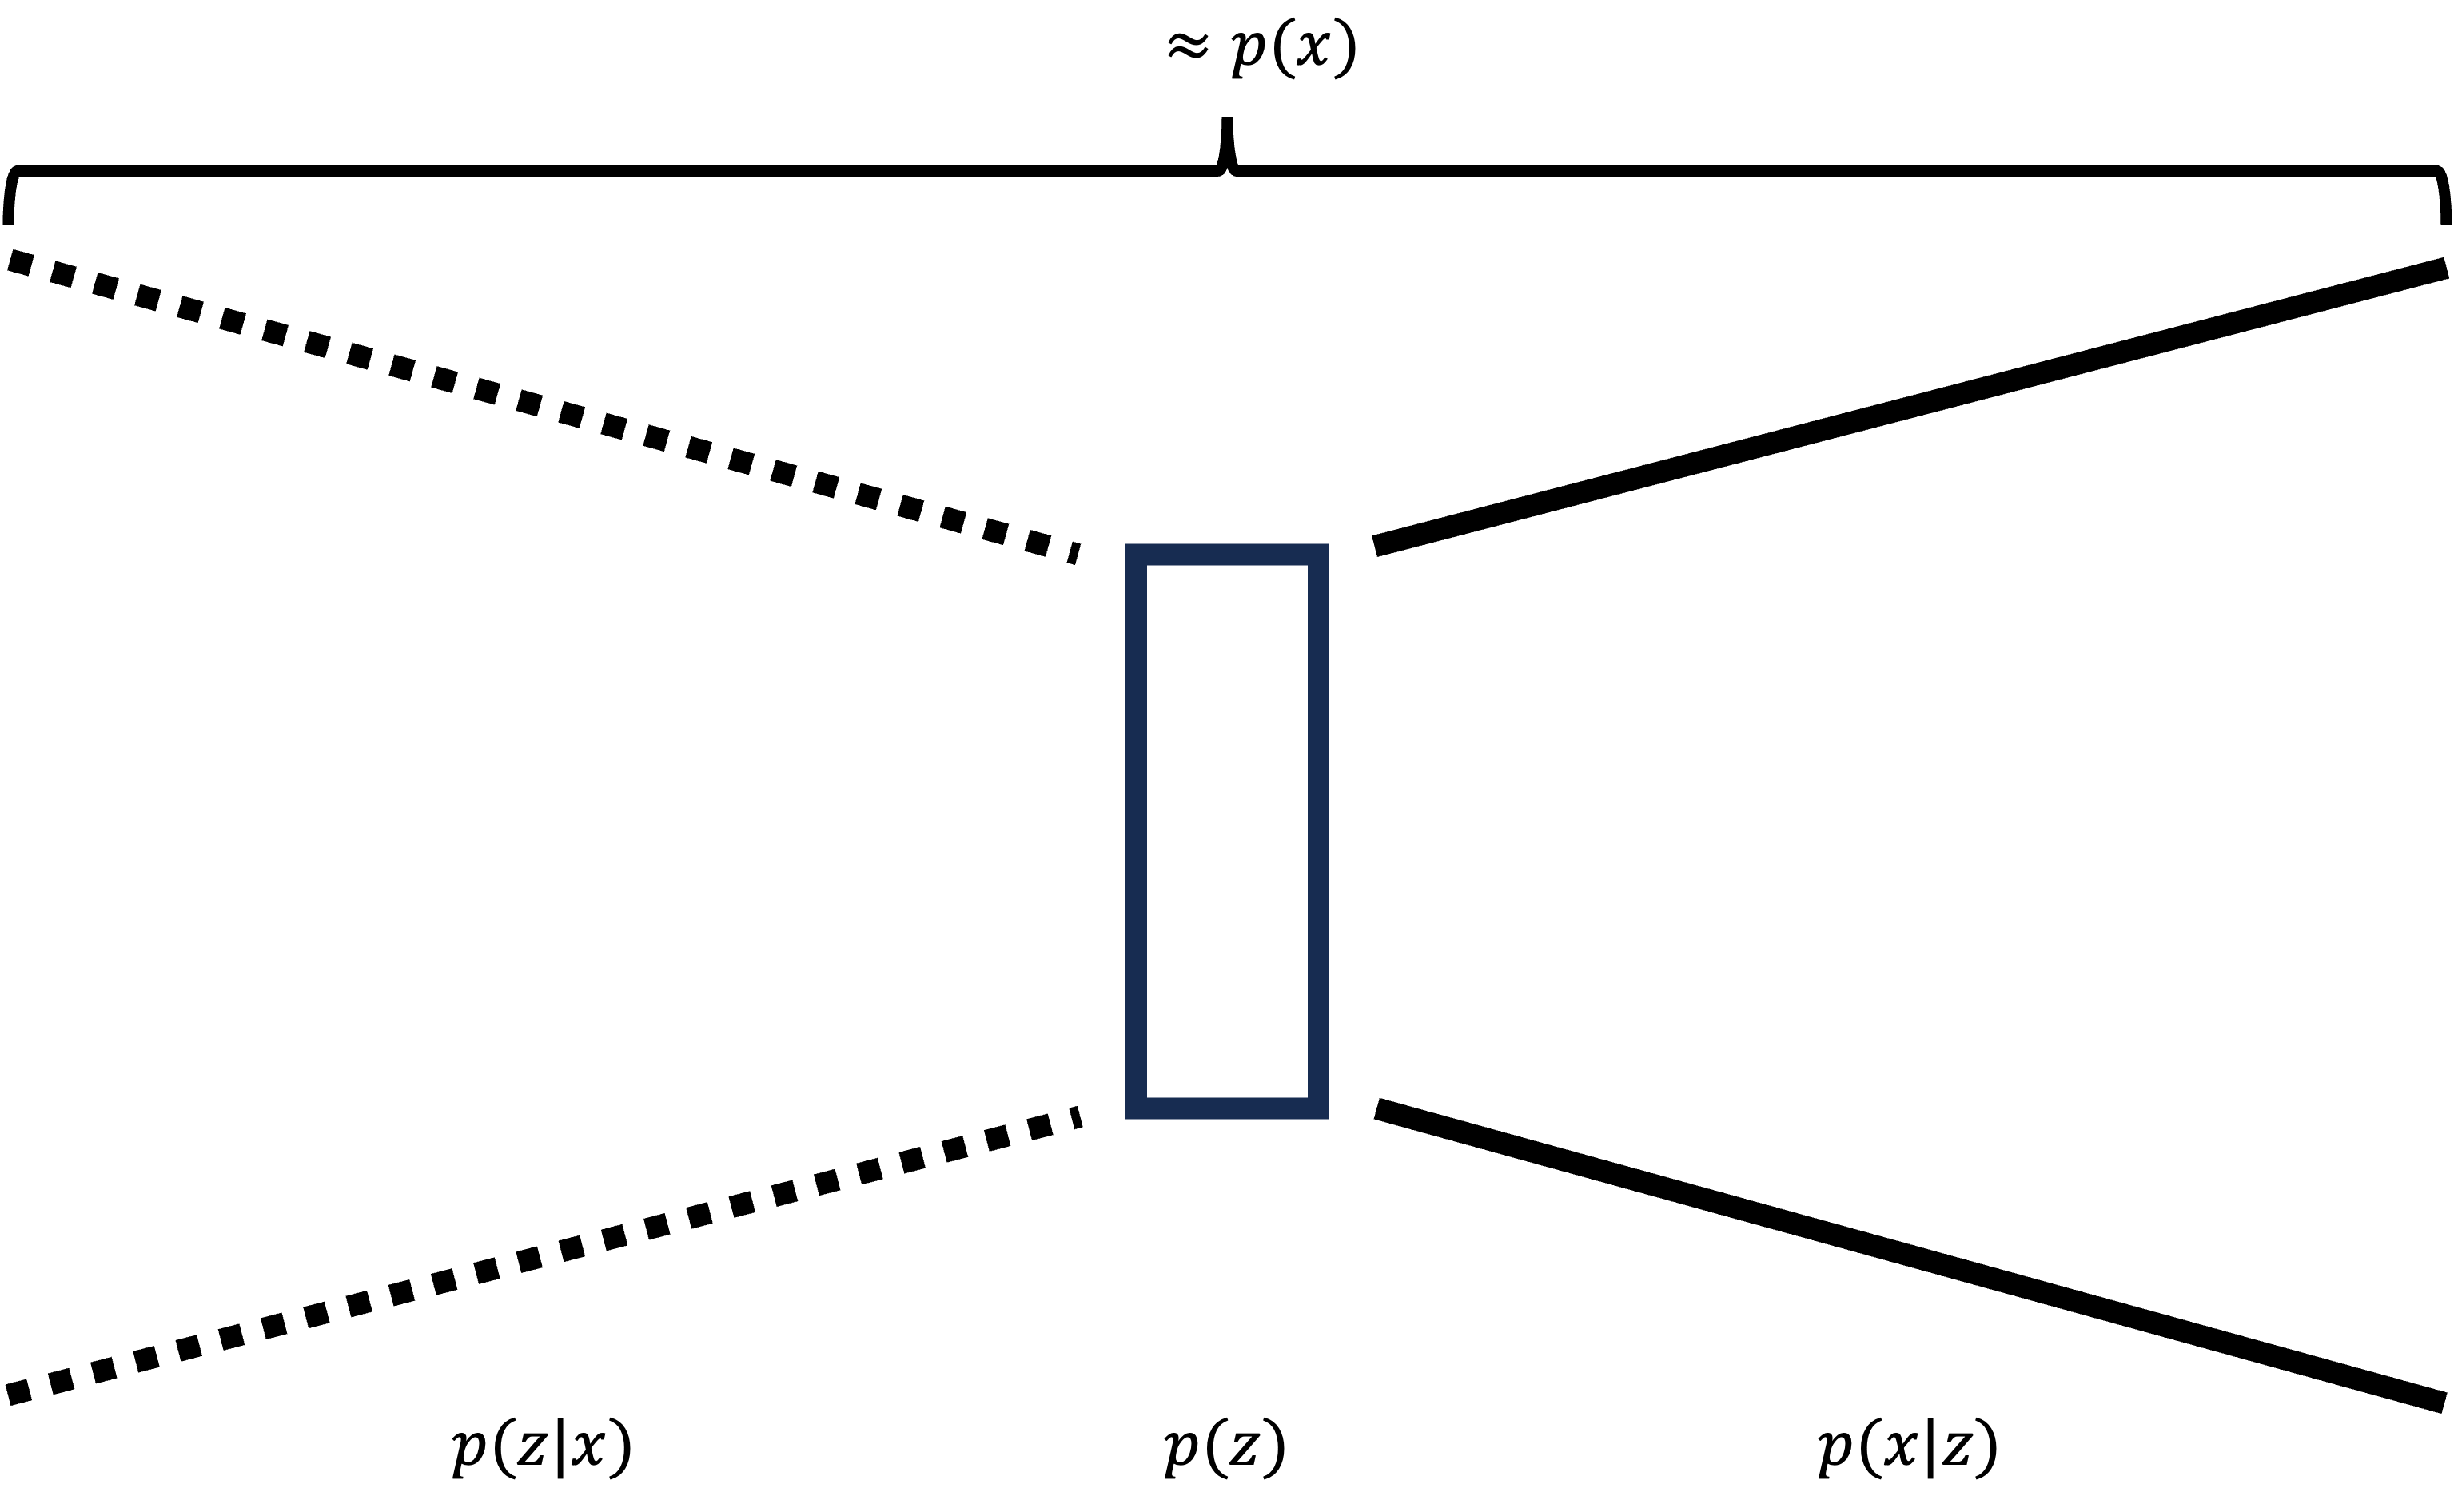
\includegraphics[width=.5\textwidth]{images/vae.png}
    \caption[VAE schematic]{VAE schematic: $p(x)$ is approximated through a latent variable model where posterior and likelihood are modeled with neural networks and the prior on the latent variable is modeled through a simple parameterized distribution (often Gaussian). The hope is, that after training, sampling from $p(z)$ and passing it through the neural network $p_{\theta_{NN}}(x|z)$, is the same as sampling from $p(x)$.}
    \label{fig:vae}
\end{figure}
Figure
The name of the VAE stems from the Autoencoder, a neural network that learns to recreate its output through an encoder with a bottleneck and a decoder, thereby learning a compressed representation of the data at the bottleneck and Fig.~\ref{fig:vae} illustrates the connection.~\autocite{https://doi.org/10.1002/aic.690370209} Autoencoders bear similarity to other dimension reduction methods like Principal Component Analysis (PCA) and therefore were first published under the name \textit{Nonlinear principal component analysis}.
\subsection{KL Divergence and Variational Lower Bound}
In VAEs, the encoder $p_{\theta}(z|x)$ needs to approximate the true posterior $p(z|x)$ and sampled data should look like it was sampled from $p(x)$. This requires a measure that can compare the similiarity between two probability distributions. One such heavily used measure is the KL (Kullback-Leibler) divergence, formulated for the posterior and its approximation as
\begin{equation}
    \label{eq:kldivergence}
    KL\left[p_{\theta}(z|x) || p(z|x)\right] = \int \log \frac{p_{\theta}(z|x)}{p(z|x)} p_{\theta}(z|x) dz = \mathbb{E}_{z\sim p_{\theta}(z|x)}\left[\log \frac{p_{\theta}(z|x)}{p(z|x)}\right].
\end{equation}
The KL divergence has the properties of being strictly non-negative and only being 0 if the two distributions are equal, but the proofs of those properties are omitted in this work.

The problem with the KL divergence in Eq.~\ref{eq:kldivergence} is that the true posterior is unknown. We will therefore introduce a loss function called ELBO (evidence lower bound) or VLB (variational lower bound) that automatically makes sure that the KL divergence between the parameterized posterior and the true posterior is minimized, without knowing $p(z|x)$. For understanding the ELBO, it is important to note that the marginal log-likelihood can be written as follows (derivation in the appendix):
\begin{align}
    \log p_{\theta}(x) & = \mathbb{E}_{z\sim p_{\theta_{NN}}(z|x)}\left[\log \frac{p_{\theta_{NN}}(x|z) p_{\theta_z}(z)}{p_{\theta_{NN}}(z|x)}\right] + KL\left[p_{\theta_{NN}}(z|x)||p(z|x)\right]
\end{align}
From the properties of the KL divergence we know that the second term on the right hand side is strictly non-negative, this means that the first term on the right hand side offers a lower bound to the log-likelihood of the data and the difference between that first term and the log-likelihood of the data is exactly the KL divergence that we wanted to minimize in Eq.~\ref{eq:kldivergence}. The relationship is also illustrated in Fig.~\ref{fig:elbo}.
\begin{equation}
    \label{eq:elbo}
    \log p_{\theta}(x) \geq \mathbb{E}_{z\sim p_{\theta_{NN}}(z|x)}\left[\log\frac{p_{\theta_{NN}}(x|z) p_{\theta_z}(z)}{p_{\theta_{NN}}(z|x)}\right]
\end{equation}
\begin{figure}[h]
    \centering
    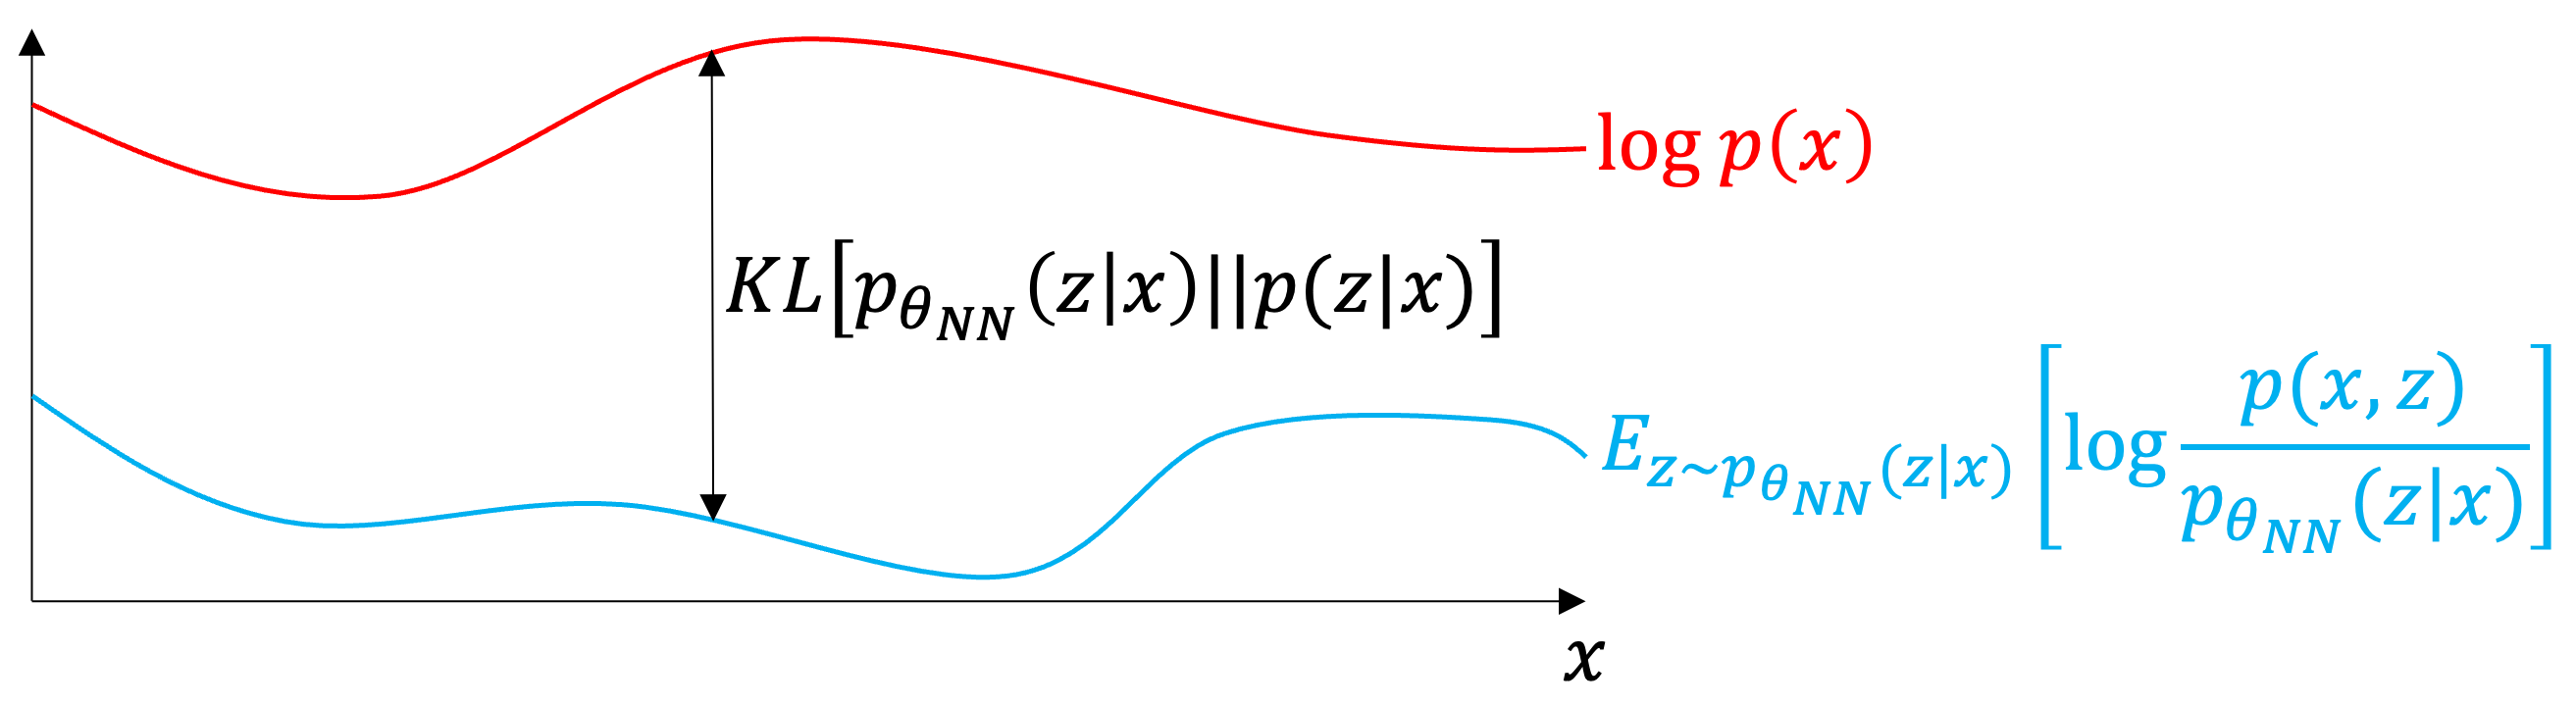
\includegraphics[width=.5\textwidth]{images/elbo.png}
    \caption[Illustration of the ELBO/VLB]{Illustration of the ELBO/VLB: The ELBO term gives a lower bound to the log-likelihood since the KL divergence is strictly non-negative. By maximizing the ELBO term, the KL divergence term is implicitly minimized and ELBO term converges towards the log-likelihood.}
    \label{fig:elbo}
\end{figure}
This means that, if we could maximize the term ELBO term from Eq.~\ref{eq:elbo} it would not only approach the log-likelihood, but simultaneously make sure that the estimated posterior converges to the true posterior. Luckily, for the parameterization of the VAE, the ELBO term can be split into two interpretable parts for optimization.
\begin{align}
    \mathbb{E}_{z\sim p_{\theta_{NN}}(z|x)}\left[\log\frac{p_{\theta_{NN}}(x|z) p_{\theta_z}(z)}{p_{\theta_{NN}}(z|x)}\right] & = \mathbb{E}_{z\sim p_{\theta_{NN}}(z|x)}\left[\log p_{\theta_{NN}}(x|z)\right] - \mathbb{E}_{z\sim p_{\theta_{NN}}(x|z)}\left[\log \frac{p_{\theta_{z}}(z)}{p_{\theta_{NN}}(z|x)}\right]                                        \\
                                                                                                                              & = \underbrace{\mathbb{E}_{z\sim p_{\theta_{NN}}(z|x)}\left[\log p_{\theta_{NN}}(x|z)\right]}_{\text{reasonable reconstruction}} - \underbrace{KL \left[p_{\theta_{NN}}(z|x)||p_{\theta_{z}}(z)\right]}_{\text{correct encoding}}
\end{align}
Maximizing the first part makes sure that the decoder reconstructs reasonable samples from the latent distribution, minimizing the second makes sure that the encoder transforms the training data into our chosen prior over the latents $z$ (usually Gaussian, as mentioned before). The reconstruction term is trivially maximized by minimizing some loss between input and output and if the prior $p(z)$ is chosen to be a Gaussian $p_{\theta_{z}}(z)$, then the KL divergence has a closed form, the derivation of which is omitted.~\autocite{mreasykldivergence}
\begin{equation}
    D_{KL}(p||q) = \frac{1}{2}\left[\log\frac{|\Sigma_q|}{|\Sigma_p|} - k + (\boldsymbol{\mu_p}-\boldsymbol{\mu_q})^T\Sigma_q^{-1}(\boldsymbol{\mu_p}-\boldsymbol{\mu_q}) + tr\left\{\Sigma_q^{-1}\Sigma_p\right\}\right]
\end{equation}

In the next section, the DDPM (diffusion denoising probabilistic model) will be introduced, which is the model architecture used throughout this work. As will be clear shortly, DDPMs can be viewed as a chained VAE that uses a sequence of latent spaces. This is an arguably easier learning problem, since the neural network does not have to map directly from noise to samples, but can do so in an iterative process over many steps.

\section{Diffusion Denoising Probabilistic Models}
Diffusion Denoising Probabilistic Models (DDPMs or Diffusion Models) are a generative model that learn the distribution of images in a training set. During training, sample images are gradually destroyed by adding noise over many iterations and a neural network is trained, such that these steps can be inverted.

As the name suggests, image content is diffused in timesteps, therefore we use the random variable $\bm{x}_0$ to represent our original training images, $\bm{x}_t$ for (partially noisy) images at an intermediate timestep and $\bm{x}_T$ for images at the end of the process where all information has been destroyed, and the distribution $q(\bm{x}_T)$ largely follows an isotropic Gaussian distribution.

The goal is to train a network that creates a less noisy image $\bm{x}_{t-1}$ from $\bm{x}_t$. If this is achieved over the whole training distribution, then sampling new $\bm{x}_T$ and passing and iteratively denoising it, should be the same as sampling $q(\bm{x}_0)$ directly.

\subsection{Forward Diffusion Process}
In order to derive a training objective it is important to understand the workings of the \textit{forward diffusion process}. During this process, i.i.d (independent and identically distributed) Gaussian noise is applied to the image over many discrete timesteps. A \textit{variance schedule} defines the means and variances ($\sqrt{1-\beta}$ and $\beta$) of the added noise at every timestep.~\autocite{ho2020denoising} The whole process can be expressed as a Markov chain (depicted in Fig.~\ref{fig:forward_diffusion}), with the factorization
\begin{align}
    \label{eq:forwardprocess}
    q(\bm{x}_{0:T})            & = q(\bm{x}_0) \prod_{t=1}^{T} q(\bm{x}_{t}|\bm{x}_{t-1}) &  & \text{(joint distribution)}       \\
    q(\bm{x}_{0:T}|\bm{x}_{0}) & = \prod_{t=1}^{T} q(\bm{x}_{t}|\bm{x}_{t-1})             &  & \text{(forwarding single sample)}
\end{align}
where the transition distributions $q(\bm{x}_t|\bm{x}_{t-1}) = \mathcal{N}(\sqrt{1-\beta_t} \bm{x}_{t-1}, \beta_t I)$ and we used the shorthand notation $\bm{x}_{0:T} = \bm{x}_{0},\dots,\bm{x}_{T}$. An example of iterative destruction of an image by this process is shown in Fig.~\ref{fig:forward_naoshima}.

\begin{figure}[h]
    \centering
    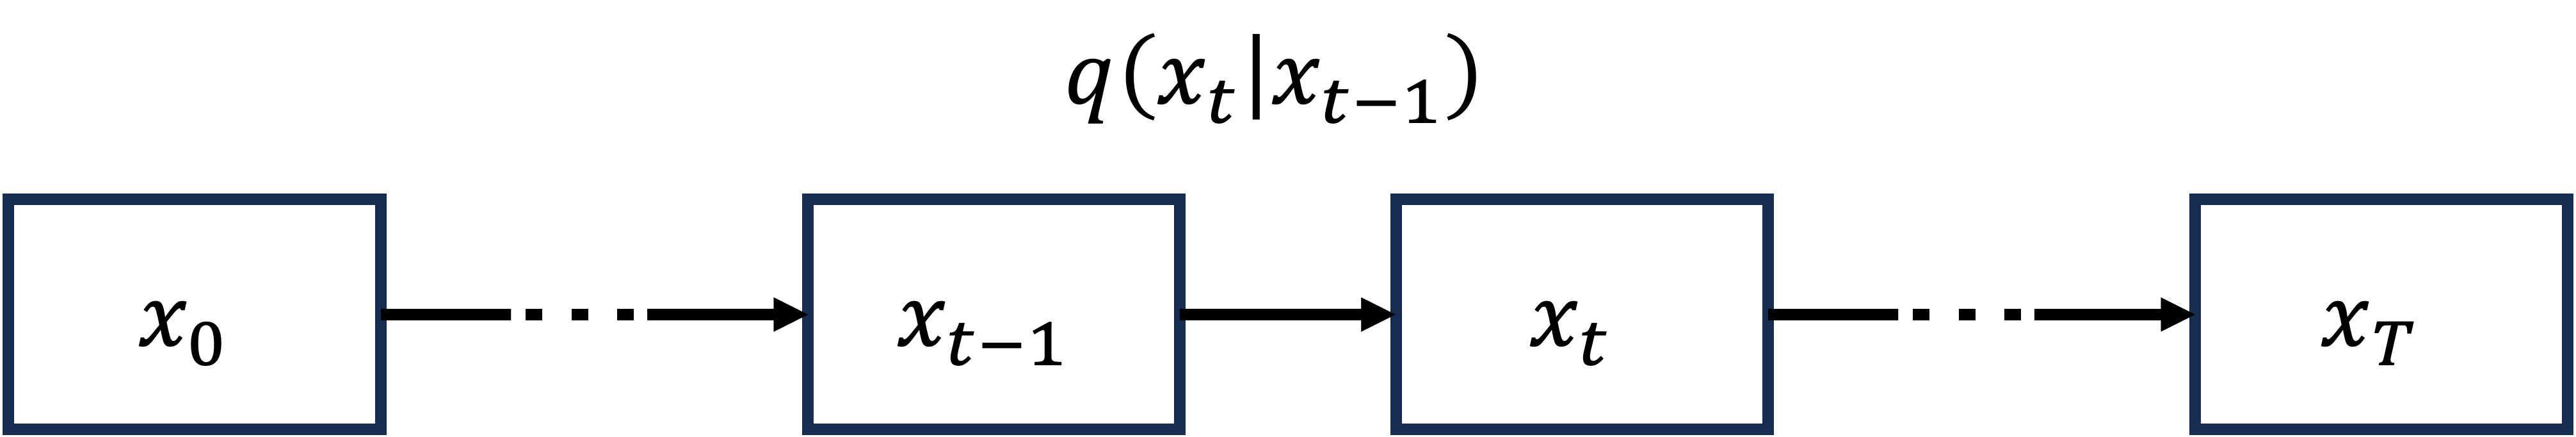
\includegraphics[width=.5\textwidth]{images/forward_diffusion.png}
    \caption[Markov Chain Interpretation of Forward Diffusion Process]{Markov Chain Interpretation of Forward Diffusion Process: An image is iteratively destroyed by adding normally distributed noise,
        according to a schedule. This represents a Markov process with the transition probability $q(\bm{x}_t|\bm{x}_{t-1})$.}
    \label{fig:forward_diffusion}
\end{figure}

\begin{figure}[h]
    \centering
    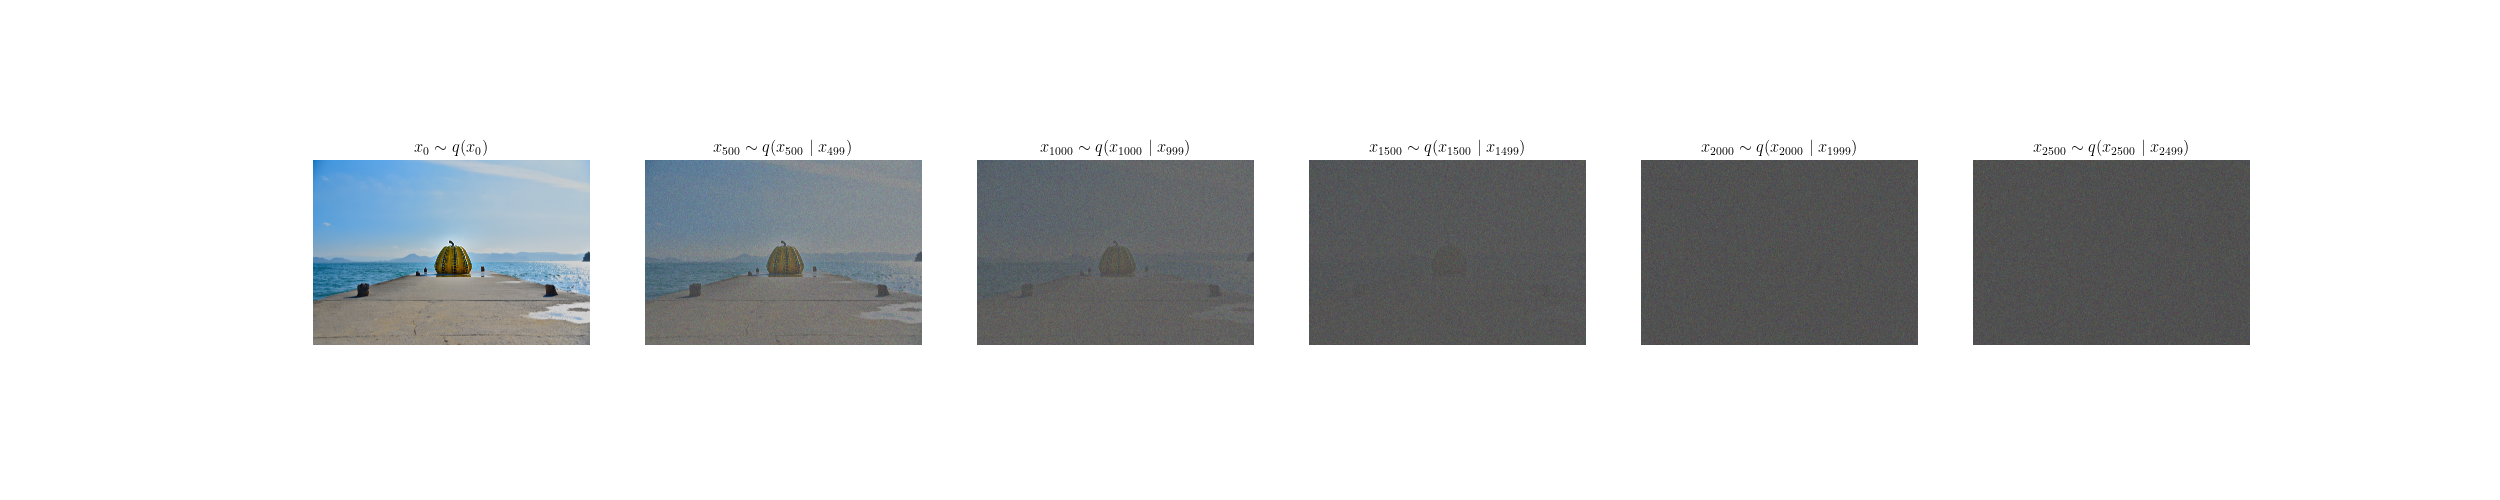
\includegraphics[width=\textwidth]{images/forward_naoshima.png}
    \caption[Example of Iterative Image Destruction through Forward Diffusion Process]{Example of Iterative Image Destruction through Forward Diffusion Process:
        The indices give the time step in the iterative destruction process, where $\beta$ was created according to a linear noise variance schedule (5000 steps from in the 0.001 to 0.02 range and picture resolution of 4016$\times$6016 pixels).}
    \label{fig:forward_naoshima}
\end{figure}

Gladly it is not necessary to sample noise again and again in order to arrive at $\bm{x}_t$, since Ho et al. derived a closed-form solution to the sampling procedure.~\autocite{ho2020denoising} For this, the variance schedule is first reparameterized as $1-\beta = \alpha$
\begin{equation}
    q(\bm{x}_t | \bm{x}_{t-1}) = \mathcal{N}(\sqrt{\alpha_t} \bm{x}_{t-1}, (1-\alpha_t) \bm{I})
    \label{eq:forward_alpha}
\end{equation}
and the closed-form solution for $q(\bm{x}_t|\bm{x}_0)$ is derived by introducing the cumulative product $\bar{\alpha}_t = \prod_{s=1}^{t}\alpha_s$ as
\begin{equation}
    q(\bm{x}_t|\bm{x}_0) = \mathcal{N}(\sqrt{\bar{\alpha}_t}\bm{x}_0, (1-\bar{\alpha}_t)\bm{I})
    \label{eq:forward_alphadash}
\end{equation}
The derivation that leads from Eq.~\ref{eq:forward_alpha} to Eq.~\ref{eq:forward_alphadash} is left to appendix~\ref{app:forward}.

A choice of $\bar{\alpha}_t \in [0,1]$ in above parameterizaiton ensures that the variance does not explode in the process, but that the SNR (signal-to-noise-ratio) still goes to 0 by gradually attenuating the means, corresponding to the original image. Thanks to the reparameterization with $\bar{\alpha}_t$, the forward process is also not restricted anymore to discrete timesteps, but a continuous schedule can be used.~\autocite{kingma2023variational,song2021scorebased}

The process of information destruction is dependent on the chosen variance schedule, the number of steps and the image size. Beyond the most simple case -- a constant variance over time -- Ho et al. opted for the second most simple option, a linear schedule, where the variance $\beta_t$ grows linearly in $t$.~\autocite{ho2020denoising} Nichol et al. later found that a cosine-based schedule gives better results on lower resolution images, since it does not destruct information quite as quickly, making it more informative in the last few timesteps. They also mention that their cosine schedule is purely based on intuition and they expect similar functions to perform equally well.~\autocite{nichol2021improved}  Own experiments exploring above mentioned parameters are explained in~\ref{sec:forward_diff_experiments} and plots of the two different variance schedules are visible in Fig.~\ref{fig:alphadash}.

\subsection{Reverse Diffusion Process}
As mentioned before DDPMs can be viewed as latent space models in a similar way that Generative Adversarial Nets or Variational Autoencoders can.~\autocite{goodfellow2014generative,kingma2013autoencoding} In DDPMs the reverse process is essentially again a Markov chain and can therefore again be factorized as
\begin{equation}
    \label{eq:reverseprocess}
    q(\bm{x}_{0:T}) = q(\bm{x}_T) \prod_{t=T}^{1} q(\bm{x}_{t-1}|\bm{x}_{t})
\end{equation}
where we start from $\bm{x}_T\sim\mathcal{N}(0,\bm{I})$. This means that the network does not learn to approximate the full inversion, but rather just the transition probabilities $q(\bm{x}_{t-1}|\bm{x}_{t})$ in the chain, which are transitions between several intermediate latent distributions. During training, we will need to condition the inversion on a training sample, where the Markov properties of the reverse process will no longer hold. In the appendix, it is shown that the inversion is also Gaussian, we therefore train a neural network to approximate
\begin{equation}
    \label{eq:reverseapprox}
    q(\bm{x}_{t-1} | \bm{x}_t) \approx p_{\theta}(\bm{x}_{t-1} | \bm{x}_t) = \mathcal{N}(\bm{\mu}_{\theta}(\bm{x}_t, t),\bm{\Sigma}_{\theta}(\bm{x}_t, t)).
\end{equation}

\subsection{Loss Functions}
The combination of forward $q(\bm{x}_T|\bm{x}_0)$ and reverse process $q(\bm{x}_0|\bm{x}_T)$ can be viewed as a chain of VAEs and we can again formulate a variational lower bound objective like before. The lengthy derivation of the ELBO for the DDPM is omitted in this work, but can be looked up in the Calvin Luo's work.~\autocite{luo2022understanding} The final form is similar to the one from the VAE, with a reconstruction term and a prior matching term, but with additional terms that match the intermediate latents.
\begin{align}
    \log p_{\theta}(x) & \geq \underbrace{\mathbb{E}_{q(x_1|x_0)} \left[ \log p_{\theta}(x_0|x_1) \right]}_{\text{reasonable reconstruction}}          \\
                       & - \underbrace{KL \left[ q(x_T|x_0) || p(x_t) \right]}_{\text{correct encoding}}                                               \\
                       & - \sum_{t=2}^{T} \underbrace{KL \left[ q(x_{t-1}|x_{t},x_0) || p_{\theta}(x_{t-1}|x_{t}) \right]}_{\text{denoising matching}}
\end{align}
The term $q(x_{t-1}|x_{t},x_0)$ is the true reverse process, conditioned on a single sample. This term comes to be when substituting the posterior transitions $p(x_t|x_{t-1})$ with $p(x_t|x_{t-1}, x_0)$, which is allowed since the Markov property states that $x_t$ only depends on $x_{t-1}$. The natural choice for the denoising matching term would be $KL\left[ q(x_t|x_{t-1}) || p_{\theta}(x_t|x_{t+1}) \right]$, but this has higher variance and is therefore harder to estimate.~\autocite{ho2020denoising} Due to the DDPM usually having 1000 or more timesteps, the ELBO is dominated by the third term. For this reason the first term is usually not used during optimization, since it can only be estimated using Monte Carlo sampling. While it is not used for optimization, it can be useful for evaluating the performance of a trained model. The second term is parameter-free therefore also not used for optimization. It should anyway be zero if the parameterization of the forward process is correct, which means that forward diffused samples get close to our chosen latent prior $p(x_T) = \mathcal{N}(0,\bm{I})$. As mentioned before, $p_{\theta}(x_{t-1}|x_t)$ is also Gaussian and since it was decided to fix the variances of the transitions to a fixed schedule, the variances of the inversion are often fixed as well and only the means are learned. When looking at the formula for the KL divergence between two Gaussians (Eq.~\ref{eq:kldivergence}) with fixed diagonal covariance matrices, one can derive that it reduces to a mean squared error between the distributional means.~\autocite{luo2022understanding}
\begin{equation}
    \hat{\theta} = \argmin_{\theta} KL \left[ q(x_{t-1}|x_{t},x_0) || p_{\theta}(x_{t-1}|x_{t}) \right] = \argmin_{\theta} \frac{1}{2\beta(t)^2} \left[ || \mu_{\theta} - \mu_{q} ||_2^2 \right]
\end{equation}
Ho et al.~\autocite{ho2020denoising} found that it works best, if the network is trained to predict the noise in the image directly and the means are then found through reparameterization
\begin{equation}
    \mu_{\theta}(x_t,t) = \frac{1}{\sqrt{\alpha_t}}x_t - \frac{1-\alpha_t}{\sqrt{1-\bar{alpha}_t}\sqrt{\alpha_t}}\hat{\epsilon}_{\theta}(x_t,t)
\end{equation}
which transforms the loss from before into
\begin{equation}
    \hat{\theta} = \argmin_{\theta}\frac{1}{2\beta(t)^2} \frac{(1-\alpha_t)^2}{(1-\bar{alpha}_t)\alpha_t} \left[ || \epsilon_0 - \hat{\epsilon}(x_t, t)  ||_2^2 \right]
\end{equation}


Another simplification is usually taken and $p_{\theta}(\bm{x}_{t-1} | \bm{x}_t)$ only approximates the means $\bm{\mu}_{\theta}$ and not the variances. For small enough timesteps, the means determine the transitional distributions much stronger than the variances. The network is furhter usually trained to not predict the means directly, but the noise and the means are then determined through a reparameterization.~\autocite{ho2020denoising,nichol2021improved}

\section{Guided Diffusion}
\subsection{Classifier Guidance}
Classifier guidance as termed by Nichol et al. introduces a data consistency term $p(s|x_t)$ in the form of a classifier trained on noisy images, where $s$ is the random variable expressing if an image belongs to a certain class.~\autocite{dhariwal2021diffusion,sohldickstein2015deep} Conditioning on a classifier is sucessfully used by taking gradient ascent steps not only in the direction that maximizes the prior $p(x)$ in a DDPM $\nabla_{x_t} \log p(x_t)$, but also the direction of this conditioning term $\nabla_{x_t} \log p(s|x_t)$. In total, this is equal to Eq.~\ref{eq:mapestimation}
\begin{equation}
    x_{t+1} = \underbrace{x_{t} + \nabla_{x_t} \log p(x_t)}_{x'_{t+1}} + \lambda \nabla_{x_t} \log p(s|x_t)
\end{equation}
with $x'_{t+1}$ being the prediction of the reverse diffusion steps before any conditioning and $\lambda$ an arbitrary factor determining the strength of the guidance.

\subsection{Image-Guided Diffusion}
\label{sec:imageguidance}
Knowledge of the forward process makes it possible to inject information from target images into the latent space where they can be fused with prediction. Lugmayr et al. make use of this for the tasks of image inpainting by always substituting the known image areas during the reverse diffusion.~\autocite{lugmayr2022repaint}
\begin{equation}
    x_{t} = \mathcal{M}^{-1}(x_t) + \mathcal{M}(s_t)
\end{equation}
They further enhance their approach using a resampling strategy, that gives the model more time to harmonize the semantics of the image. An example of such a resampling schedule can be seen in Fig.~\ref{fig:stepsplot}.

Choi et al. also substitute parts of the image in order to guide the inverse diffusion process, but they substitute low-frequency information by using linear filters.~\autocite{choi2021ilvr}
\begin{equation}
    x_{t} = \phi(s_{t}) + (I - \phi) (x_{t})
\end{equation}
They demonstrate strong performance in image translation tasks, e.g. from painting to photo-realistic image.
%% ----------------------------------------------------------------------------
% BIWI SA/MA thesis template
%
% Created 09/29/2006 by Andreas Ess
% Extended 13/02/2009 by Jan Lesniak - jlesniak@vision.ee.ethz.ch
%% ----------------------------------------------------------------------------
\newpage
\chapter{Materials and Methods}
\section{Image Guided Diffusion}
Both, Choi et al. and Lugmayr et al. make use of unconditional DDPMs for image-guided diffusion for the tasks of image translation in the former and in-painting in the latter.~\autocite{choi2021ilvr,lugmayr2022repaint} Similarly, classifier guidance or CLIP-guidance can be used to condition unconditional DDPMs to produce samples of a specific class or to match a prompt.~\autocite{dhariwal2021diffusion} Both approaches can be combined into a flexible framework that allows the reverse diffusion process to be conditioned on any data consistency term.

\subsection{MAP Estimation for Inverse Problems}
Image reconstruction tasks, that make use of a prior over the desired reconstructed image, can be formulated as a MAP (maximum-a-posteriori) estimation problem
\begin{equation}
    \hat{x}_{MAP} = \argmax_x p(x|s) = \argmax_x \frac{p(s|x)p(x)}{p(s)}
\end{equation}
where $s \sim p(s)$ is the evidence that is provided by the measured signal, $p(x)$ is a prior on the desired reconstruction and the likelihood term $p(s|x)$ enforces a data consistency between the measured signal and the true distribution. Since maximizing $p(x|s)$ is the same as maximizing $\log(x|s)$ and $p(s)$ is independent of $\theta$, we can separate the product into a sum.
\begin{align}
    \hat{x}_{MAP} & = \argmax_x \log p(x|s)             \\ & = \argmax_x \log{\frac{p(s|x)p(x)}{p(s)}} \\
                  & = \argmax_x \log p(s|x)p(x)         \\
                  & = \argmax_x \log p(s|x) + \log p(x)
\end{align}
Such problems can be optimized using iterative optimization schemes such as gradient ascent $x_{t+1} = x_{t} + \lambda \nabla_{x} f(x, s)$, with $\lambda$ being the step length.
\begin{align}
    \label{eq:mapestimation}
    x_{i+1} = x_{i} + \nabla_{x_i} \log p(s|x_i) + \nabla_{x_i} \log p(x_i)
\end{align}
Maximizing $p(s|x)$ and $p(x)$ is in practice usually reformulated as a minimization problem that optimizes for smallest error between prediction and acquisition $\mathcal{L}(s, x)$ and enforces certain regularizers (priors) on $x$ by minimizing $\mathcal{R}(x)$. An example for MRI reconstruction could include minimizing a mean-squared-error between predicted k-space $\mathcal{F}(x)$ and acquired k-space $s$, while also minimizing the total variation in the image.~\autocite{RUDIN1992259}
\begin{equation}
    \hat{x}_{MAP} = \argmin_x \mathcal{L}(s, x) + \mathcal{R}(x) = \argmin_x \frac{1}{n}||\mathcal{F}(x) - s||_2^2 + TV(x)
\end{equation}

\subsection{DDPMs as Priors}
DDPMs approximate a data distribution over training images $p(x)$ and by the score-based formulation, they do so by learning to approximate gradients of this marginal likelihood.~\autocite{song2020generative} Sampling a DDPM therefore equals to starting in a random position and taking gradient ascent steps of the in the direction of maximizing $p(x)$ or $\log p(x)$.
\begin{equation}
    \label{eq:ddpmiteration}
    x_{t-1} = x_{t} + \nabla_{x_t} \log p(x_t)
\end{equation}
Comparing this to Eq.~\ref{eq:mapestimation} it is easy to see that this is the same as maximizing for a prior in a reconstruction task and we can introduce a data consistency that works similarly to classifier-guidance~\autocite{dhariwal2021diffusion}, but makes the reverse diffusion process converge to acquired data instead of an easily-classified image.
\begin{align}
    \hat{x} & = \argmax_x \log p(x) + \log p_{\theta}(c|x)        &  & \text{(classifier-guidance)}       \\
            & = \argmax_x \log p(x) + \log p(s|x)                 &  & \text{(data-consistency guidance)} \\
            & = \argmax_x \log p(x) + \argmin_x \mathcal{L}(s, x) &  & \text{(for $\mathcal{L} \geq 0$)}  \\
\end{align}
The constraint $\mathcal{L} \geq 0$ is true for the usual distance-based loss functions like mean-squared-error or the $L_1$ loss. A step in the iterative process has the following form and this algorithm will from now on be termed \textit{loss-guidance}.
\begin{equation}
    x_{t-1} = x_{t} + \nabla_{x_t} \log p(x_t) - \nabla_{x_t} \mathcal{L}(s, x)
\end{equation}
The formulation used for the task of reconstructing undersampled MRI used an MSE loss on the predicted and acquired k-space
\begin{equation}
    x_{t-1} = x_{t} + \nabla_{x_t} \log p(x_t) - g \cdot \nabla_{x_t} \frac{1}{\sum_n \mathcal{M}}||\mathcal{M} \circ \mathcal{F}(x_t) - s_0||_2^2
\end{equation}
where $g$ will be termed the \textit{guidance factor} and the MSE is is not scaled by the number of pixels in the image, but by the number of non-zero elements of the mask. This is done in order to compare guidance factors among masks with different accelerations. The guidance factor can be used to balance adherence of the outcome between prior and data consistency.

\section{Frequency Replacement}
As already stated in~\ref{sec:imageguidance}, Choi et al. guide the diffusion process by substituting low frequency content of a desired latent representation with the low-frequencies of the predicted latent space. Since they use linear filters, we are free to reformulate as follows
\begin{align}
    \label{eq:ilvr}
    x_{t} & = \phi(s_{t}) + (I - \phi) (\hat{x}_{t})        \\
          & = \hat{x}_{t} + \phi(s_{t}) - \phi(\hat{x}_{t}) \\
          & = \hat{x}_{t} + \phi(s_{t} - \hat{x}_{t})
\end{align}
where $\phi$ is a linear filter operation and $s_t$ is obtained by using the forward process on the target image.~\autocite{choi2021ilvr} With the knowledge of the gradient of the MSE
\begin{align}
    \text{MSE}              & = \frac{1}{N} (x - s)^T (x - s) \\
    \nabla_{x_t} \text{MSE} & = \frac{2}{N} (x - s)
\end{align}
the frequency replacement can also be interpreted as locally approximating the gradient of the $\nabla_{x}(\phi(s) - \phi(x_{t}))|_{s=s_t}$ and taking a step in that direction, which would correspond to the loss-guidance formulation derived earlier.

Similarly, Lugmayr et al. use a replacement strategy, which we can reformulate to the structure from Choi et al.
\begin{align}
    \label{eq:repaint}
    x_{t} & = \mathcal{M}(s_t) + \mathcal{M}^{-1}(\hat{x}_t)        \\
          & = \mathcal{M}(s_t) + (I - \mathcal{M})(\hat{x}_t)       \\
          & = \hat{x}_t - \mathcal{M}(\hat{x}_t) + \mathcal{M}(s_t) \\
          & = \hat{x}_t + \mathcal{M}(s_t - \hat{x}_t)
\end{align}
Applying these two approaches to the problem of MRI reconstruction requires calculating $s_t$ from $s_0$ which can be done in image space as $s_t = \mathcal{F}^{-1} \circ \mathcal{M} \circ \mathcal{F} (\sqrt{\bar{\alpha}_t} \mathcal{F}^{-1}(s_0) + \sqrt{1-\bar{\alpha}_t} \epsilon)$, or directly in k-space as $s_t = \mathcal{F}^{-1} \circ \mathcal{M} (\sqrt{\bar{\alpha}_t} s_0 + \sqrt{\frac{1-\bar{\alpha}_t}{2}} \epsilon)$ as experimentally derived. The scaling of the noise variance with factor $\frac{1}{2}$ was experimentally found and can be verified in Fig.~\ref{fig:kspacedistribution}. The complete formulation of the update step is therefore
\begin{align}
    x_{t} & = \hat{x}_t + \mathcal{F}^{-1}\circ\mathcal{M}\circ\mathcal{F}(\hat{x}_t) - \mathcal{F}^{-1} \circ \mathcal{M} \circ \mathcal{F} (s_t) \\
          & = \hat{x}_t + \mathcal{F}^{-1}\left(\mathcal{M}\circ\mathcal{F}(\hat{x}_t) - \mathcal{M} \circ \mathcal{F} (s_t)\right)                \\
\end{align}
which makes use of the linearity of the Fourier transform.

\section{Network Architecture}
The neural network is responsible for predicting the noise in an image and the UNet architecture has proven useful for estimating the noise in natural images, which is the context where DDPMs usually operate.~\autocite{ronneberger2015unet,ho2020denoising} The UNet implementation which was used in most experiments of this work is closely related to the original implementation by Ronneberger et al., while most other works use more sophisticated architectures that include Transformer-inspired self-attention layers for better global context awareness of the model and residual connections for faster convergence.~\autocite{vaswani2017attention,he2015deep} Saharia et al. did ablation studies on the self-attention layers and tried to replace them with other methods, such as local self-attention or dilated convolutions, but showed that the global self-attention increased both, mode coverage of the data distribution as well as sample fidelity.~\autocite{saharia2022palette} Fully convolutional architectures have the advantage that, if trained appropriately, they can generalize to different image resolutions. Such training could include random crops and downsamplings of the original images, which was the initial motivation for going with a fully-convolutional architecture. While self-attention layers were included at a later point, the additional computational cost made it difficult to reach convergence in a resonable time. Therefore the best network checkpoint, that was used in the conditioning studies of~\ref{sec:experimentsandresults}, uses the fully convolutional architecture as presented in Fig.~\ref{fig:unetconv}. This architecture sequentially increases the channels and decreases the resolution with a factor of 2 in the encoder and then upsamples the outputs of this bottleneck by incorporating additional local information through the use of skip-connections. The network is conditioned on the timestep by broadcasting a linear embedding of the Transformer-style time encoding (see Fig.~\ref{fig:timeencoding}) onto the feature dimension (channels).~\autocite{vaswani2017attention} The exact specifications can be found in Table~\ref{tab:unetlayers} and the main differences to the UNet architectures used in the DDPM literature are the following:
\begin{description}
    \item[No self-attention layers] Global self-attention increased the computational cost and often led to non-convergence of the network.
    \item[Batch norm instead of layer norm or group norm] Batch norm was not observed to cause any issues, even when training on small mini-batches, therefore it was left as it was.
    \item[No residual connections] Most other literature makes use of residual connections in the double convolutions of the encoder and decoder.
\end{description}
\begin{figure}
    \centering
    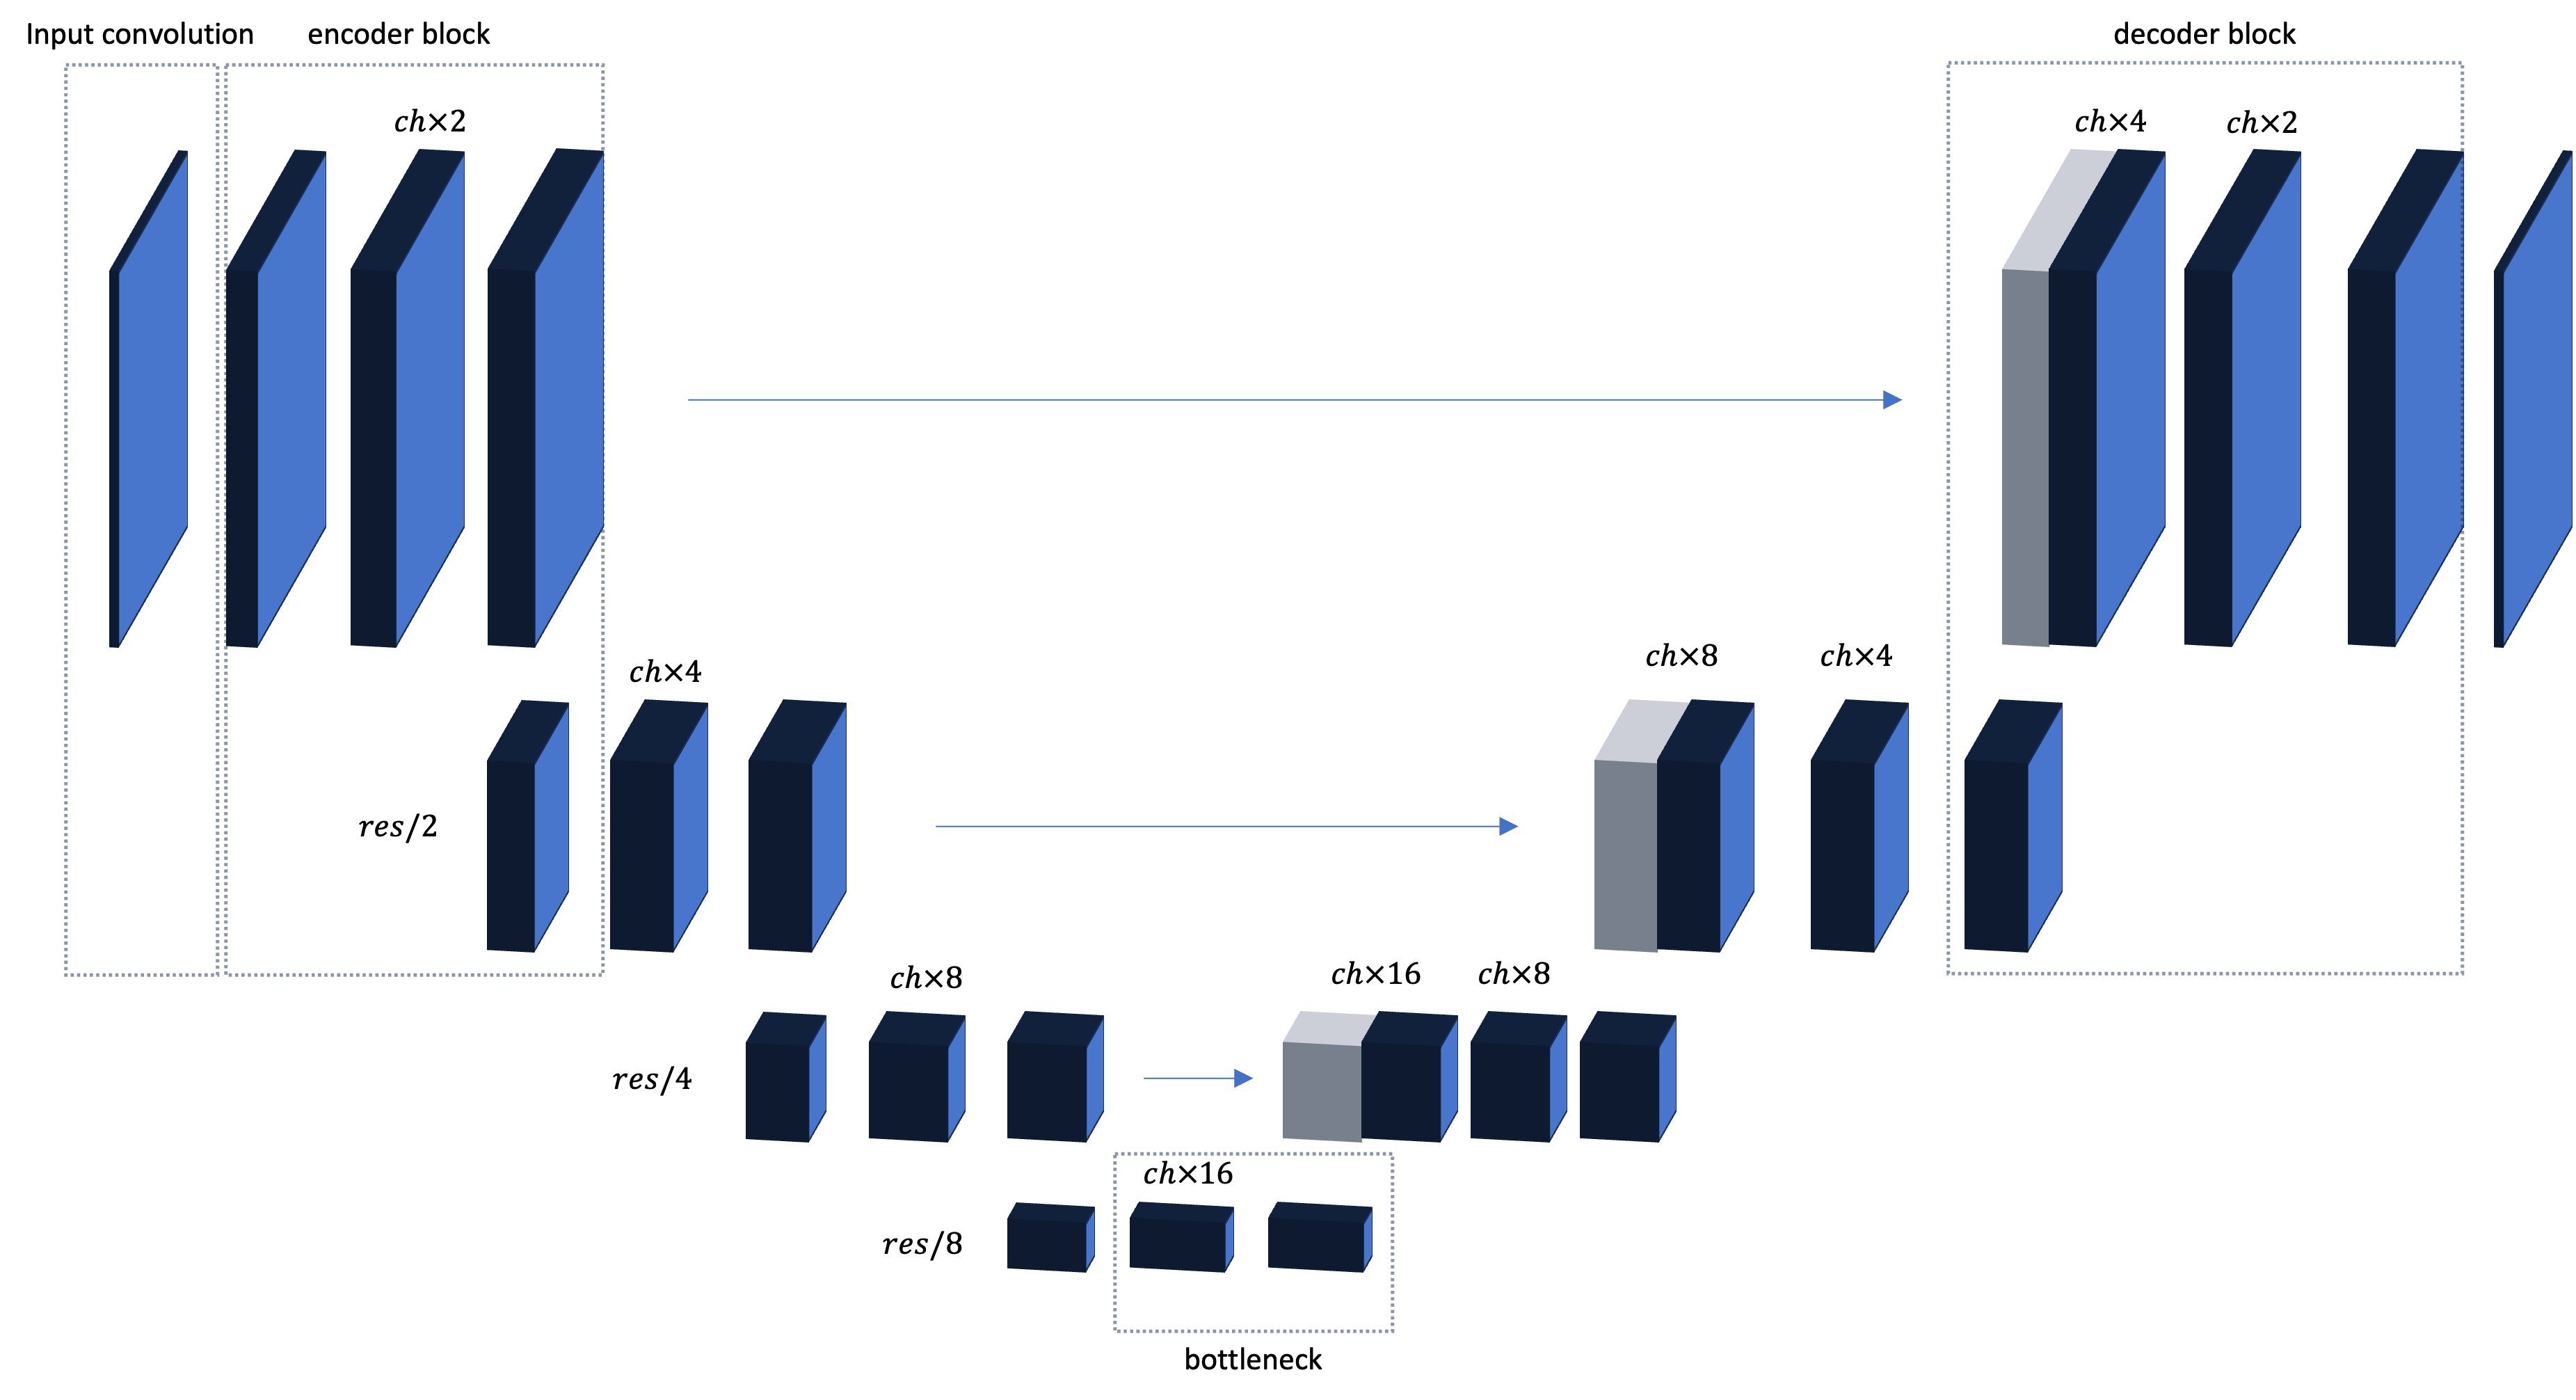
\includegraphics[width=.7\textwidth]{images/unet.png}
    \caption[Fully Convolutional UNet]{Fully Convolutional UNet architecture: An input convolution increases the channels to the number of \textit{base channels}. Consecutively a variable number of encoder blocks applies double convolutions and max pooling, before the decoder block applies transpose convolutions for upsampling and double convolutions to incorporate information from the skip connections. At the end, the output convolution maps the output back to the original number of input channels.}
    \label{fig:unetconv}
\end{figure}

\begin{table}
    \centering
    \caption[Overview over UNet Architecture]{Overview over UNet Architecture: The most successful architecture used in this work was a fully-convolutional UNet.}
    \label{tab:unetlayers}
    \begin{tabular}{l l}
        architecture part              & specification                                                                     \\
        \hline\hline
        base channels ($ch$)           & $2^n$                                                                             \\
        \hline base resolution ($res$) & $2^x \times 2^m$                                                                  \\ \hline
        convolutional block            & convolution                                                                       \\ & batchnorm\\ & activation\\ & dropout                         \\
        \hline encoder block           & convolutional block ($ch \rightarrow ch\times 2$)                                 \\ & convolutional block ($ch\times 2 \rightarrow ch\times 2$) \\ & max pool ($res\rightarrow res/ 2$) \\
        \hline decoder block           & transpose convolution ($res\times 2\rightarrow res$, $ch\times 2 \rightarrow ch$) \\ & batchnorm\\ & activation\\ & dropout \\ & skip connection stack ($ch \rightarrow ch\times 2$) \\ & convolutional block ($ch\times 2 \rightarrow ch$)\\
        \hline bottleneck              & convolutional block ($ch \rightarrow ch\times 2$)
    \end{tabular}
\end{table}

\begin{figure}
    \centering
    \
\end{figure}

\section{Slowing Down, Short-Grained Resampling \& Long-Grained Resampling}
Various approaches exist to give the reverse diffusion process more time to converge to a meaninful final prediction.

\section{Datasets}
Introductory experiments were conducted on low-resolution datasets in order to debug the model implementation and determine the best training strategies. These datasets were the well-known MNIST and CIFAR10~\autocite{mnist,cifar} in resolutions of $28\times28$ and $32\times32$ pixels respectively. Since the encoder stack relies on image resolutions of $2^n\times2^k$ with $n,k\in \mathbb{N}$, the MNIST images were upscaled to an equal $32\times32$ resolution. The MNIST dataset is a dataset containing 60'000 training images of handwritten digits 0 to 9 and CIFAR10 contains 50'000 training images distributed over 10 classes like airplane, bird, cat, etc.

The main dataset used in the experiments were the RSS (root sum of squares) reconstructions from the brain dataset in fastMRI.~\autocite{zbontar2018fastMRI} FastMRI is a collection of several MRI datasets, a large dataset of multi-coil brain scans among them. In addition to the raw multi-coil data, RSS reconstructions, combining the coils by using estimates of the sensitivity maps, are also available. Those reconstructions have very high quality and therefore this dataset provides a strong basis for useage as a prior in the reconstruction task. The RSS reconstructions provide a total of 60'090 slices of resolution $320\times320$ pixels and models were trained on downsampled versions of $256\times 256$, $128\times 128$ and $64\times 64$ pixels.

While the authors of fastMRI suggest equally-spaced masks with a fixed center fraction for brain images~\autocite{zbontar2018fastMRI}, the masks used in this work have fixed center fractions, but are randomly sampled for the higher frequencies. Three masks, and the effect they have on the samples, are shown in Fig.~\ref{fig:kspacemasking}. These masks are similar to the ones used in the experimental part.
\begin{figure}[h]
    \centering
    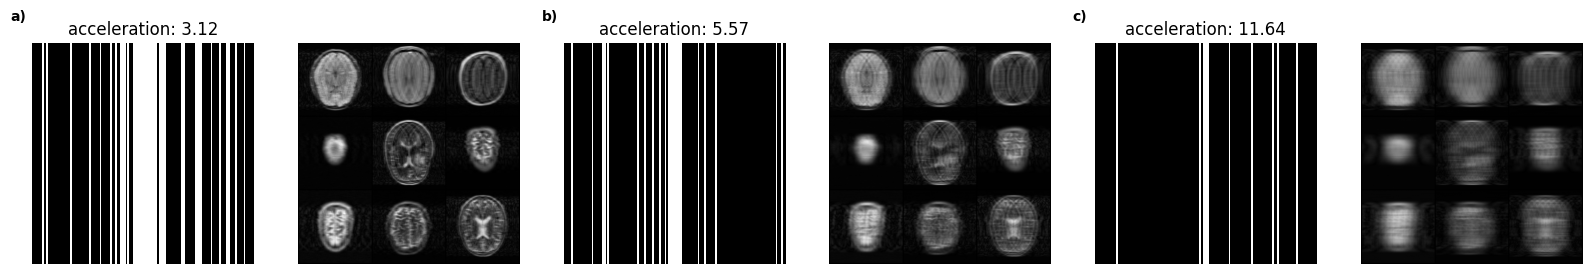
\includegraphics[width=\textwidth]{images/corruption_mask.png}
    \caption[K-Space Undersampling]{K-Space Undersampling: a) Sample of a K-Space undersampling mask with center fraction of 0.1 and a probability of 0.25 for the other frequencies, giving an effective acceleration of $\approx 3.12$. b) Effect of K-Space undersampling on samples from fastMRI dataset. While the low-frequency content is visibly intact, the undersampling of the higher frequencies causes aliasing artifacts, manifested as lines on the samples. These lines hint at the true aliases that would be generated for image space undersampling instead of randomized k-space undersampling.}
    \label{fig:kspacemasking}
\end{figure}


\section{Software Package}
In order to fully understand DDPMs it was decided to implement them from scratch instead of using repositories provided by the literature~\autocite{nichol2021improved} or by packages such as the Huggingface Diffusers library.~\autocite{huggingfacediffusers} The created repository is publicly accessible via GitHub and includes automatic documentation generation using Sphinx and GitHub Actions. Notable is also the useage of jaxtyping~\autocite{jaxtyping}, a library for type hinting tensor shapes. The repository and the documentation are accessible under the following links:
\begin{center}
    \hyperlink{https://github.com/liopeer/diffusionmodels}{https://github.com/liopeer/diffusionmodels}\\
    \hyperlink{https://liopeer.github.io/diffusionmodels/}{https://liopeer.github.io/diffusionmodels/}
\end{center}
The software package is based on PyTorch~\autocite{paszke2019pytorch} and provides model architectures as well as training utilities. These utilities include the possibility for distributed training, training logging and checkpointing, and mixed-precision training, implemented using the following frameworks.
\begin{description}
    \item[Weights \& Biases] provides an API that allows logging the model training via their website (\hyperlink{www.wandb.ai}{https://wandb.ai/}). The tool is free for students and academic researchers and automatically logs model configuration, gradients and hardware parameters in addition to user-specified logs, such as sample images, losses and inference times. When using git for versioning it also logs the most recent git commit, allowing to resume model training or to rerun an experiment with exactly the same code. When training models over several days it was very convenient to be able to observe the process from the smartphone and look at samples generated by the model.~\autocite{wandb}
    \item[PyTorch DDP (DistributedDataParallel)] parallelizes model training by launching individual processes for each GPU, or it can even launch processes across different machines. Separate processes are necessary in order to enable true parallelism that avoids Python GIL (global interpreter lock). During initialization, the model is copied across the different GPUs and during training only the gradients are synchronized and averaged across the GPUs, therefore the optimizers essentially train a local model per each process. Gradient synchronization is automatically invoked by calling \lstinline{loss.backward()}, but can be avoided by including forward and backward in the \lstinline{no_sync()} content manager, which is useful when using gradient accumulation over several micro-batches, for which the gradient synchronization would create unnecessary overhead. As part of DDP, PyTorch also offers \lstinline{DistributedSampler} (to be used with \lstinline{DataLoader}), which splits mini-batches into micro-batches and assigns them to the respective processes. For models that use batch normalization layers, DDP also offers the module \lstinline{SyncBatchNorm} and a function to recursively change all batch normalization layers to synchronized batch normalization. Synchronizing the batch normalization might be important for small micro-batch sizes or when the number of GPUs changes during training (e.g. continuing from a checkpoint).
    \item[PyTorch AMP (Automatic Mixed Precision)] provides a context manager and a function decorator that will convert certain operations to half-precision (16 bit), which gives a significant speedup for linear layers or convolutions, but keeps high precision for operations such as reductions. Half precision training might lead to underflow of gradients, because of the reduced value range and can be avoided by scaling the loss and therefore the gradients, while also inversely scaling the update step. AMP provides the \lstinline{GradScaler} class for this purpose.
\end{description}
%% ----------------------------------------------------------------------------
% BIWI SA/MA thesis template
%
% Created 09/29/2006 by Andreas Ess
% Extended 13/02/2009 by Jan Lesniak - jlesniak@vision.ee.ethz.ch
%% ----------------------------------------------------------------------------
\newpage
\chapter{Experiments and Results}
\label{sec:experimentsandresults}
Describe the evaluation you did in a way, such that an independent researcher can repeat it. Cover the following questions:
\begin{itemize}
    \item \textit{What is the experimental setup and methodology?} Describe the setting of the experiments and give all the parameters in detail which you have used. Give a detailed account of how the experiment was conducted.
    \item \textit{What are your results?} In this section, a \emph{clear description} of the results is given. If you produced lots of data, include only representative data here and put all results into the appendix.
\end{itemize}

\section{Training Models on MNIST, CIFAR and fastMRI}
In order to explore hyperparameters of the model architecture and debug the implementation it was decided to first train models on datasets considered trainable with less compute time. Two very well known datasets in computer vision that use low-resolution images are CIFAR10 and MNIST.~\autocite{cifar,mnist}
\begin{figure}[h]
    \centering
    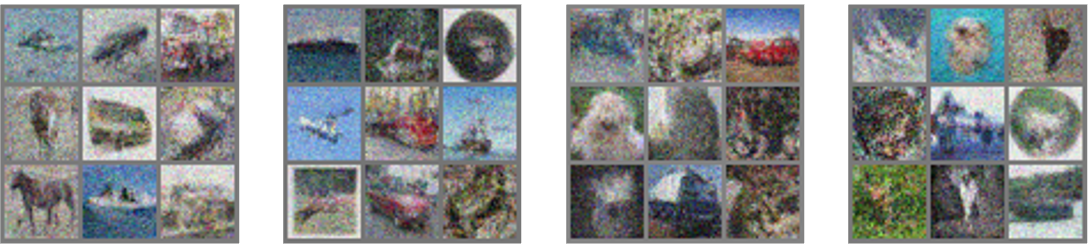
\includegraphics[width=.75\textwidth]{images/cifarsamples.png}
    \caption[Samples generated from CIFAR10]{Samples from the best performing model trained on CIFAR10 using a linear schedule: While the variance in the samples is large, suggesting that the model is able to capture the whole distribution, the samples are not completely denoised and therefore sample quality is seriously degenerated. As can be seen later, this was not observed when training on datasets where the image resolution was higher.}
    \label{fig:cifarsamples}
\end{figure}

\begin{figure}[h]
    \centering
    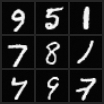
\includegraphics[width=.15\textwidth]{images/mnistsamples.png}
    \caption[Samples generated from MNIST]{Samples from the best performing model trained on MNIST}
    \label{fig:mnistsamples}
\end{figure}

Unconditional sampling was performed in order to verify the sample quality and whether the model was able to capture the main modes of the training data distribution. For a quantitative analysis of sample quality and mode coverage/log-likelihood of trained models Nichol et al. use FID score and Monte-Carlo log-likelihood estimates. FID requires the training of an additional classifier network, which only makes sense on standardized datasets with class labels such as ImageNet or CIFAR.~\autocite{imagenet, cifar} Pretrained classifiers are available for these datasets, which makes scores comparable among different generative models. The fastMRI dataset is not meant for classification tasks, therefore
\begin{figure}[h]
    \centering
    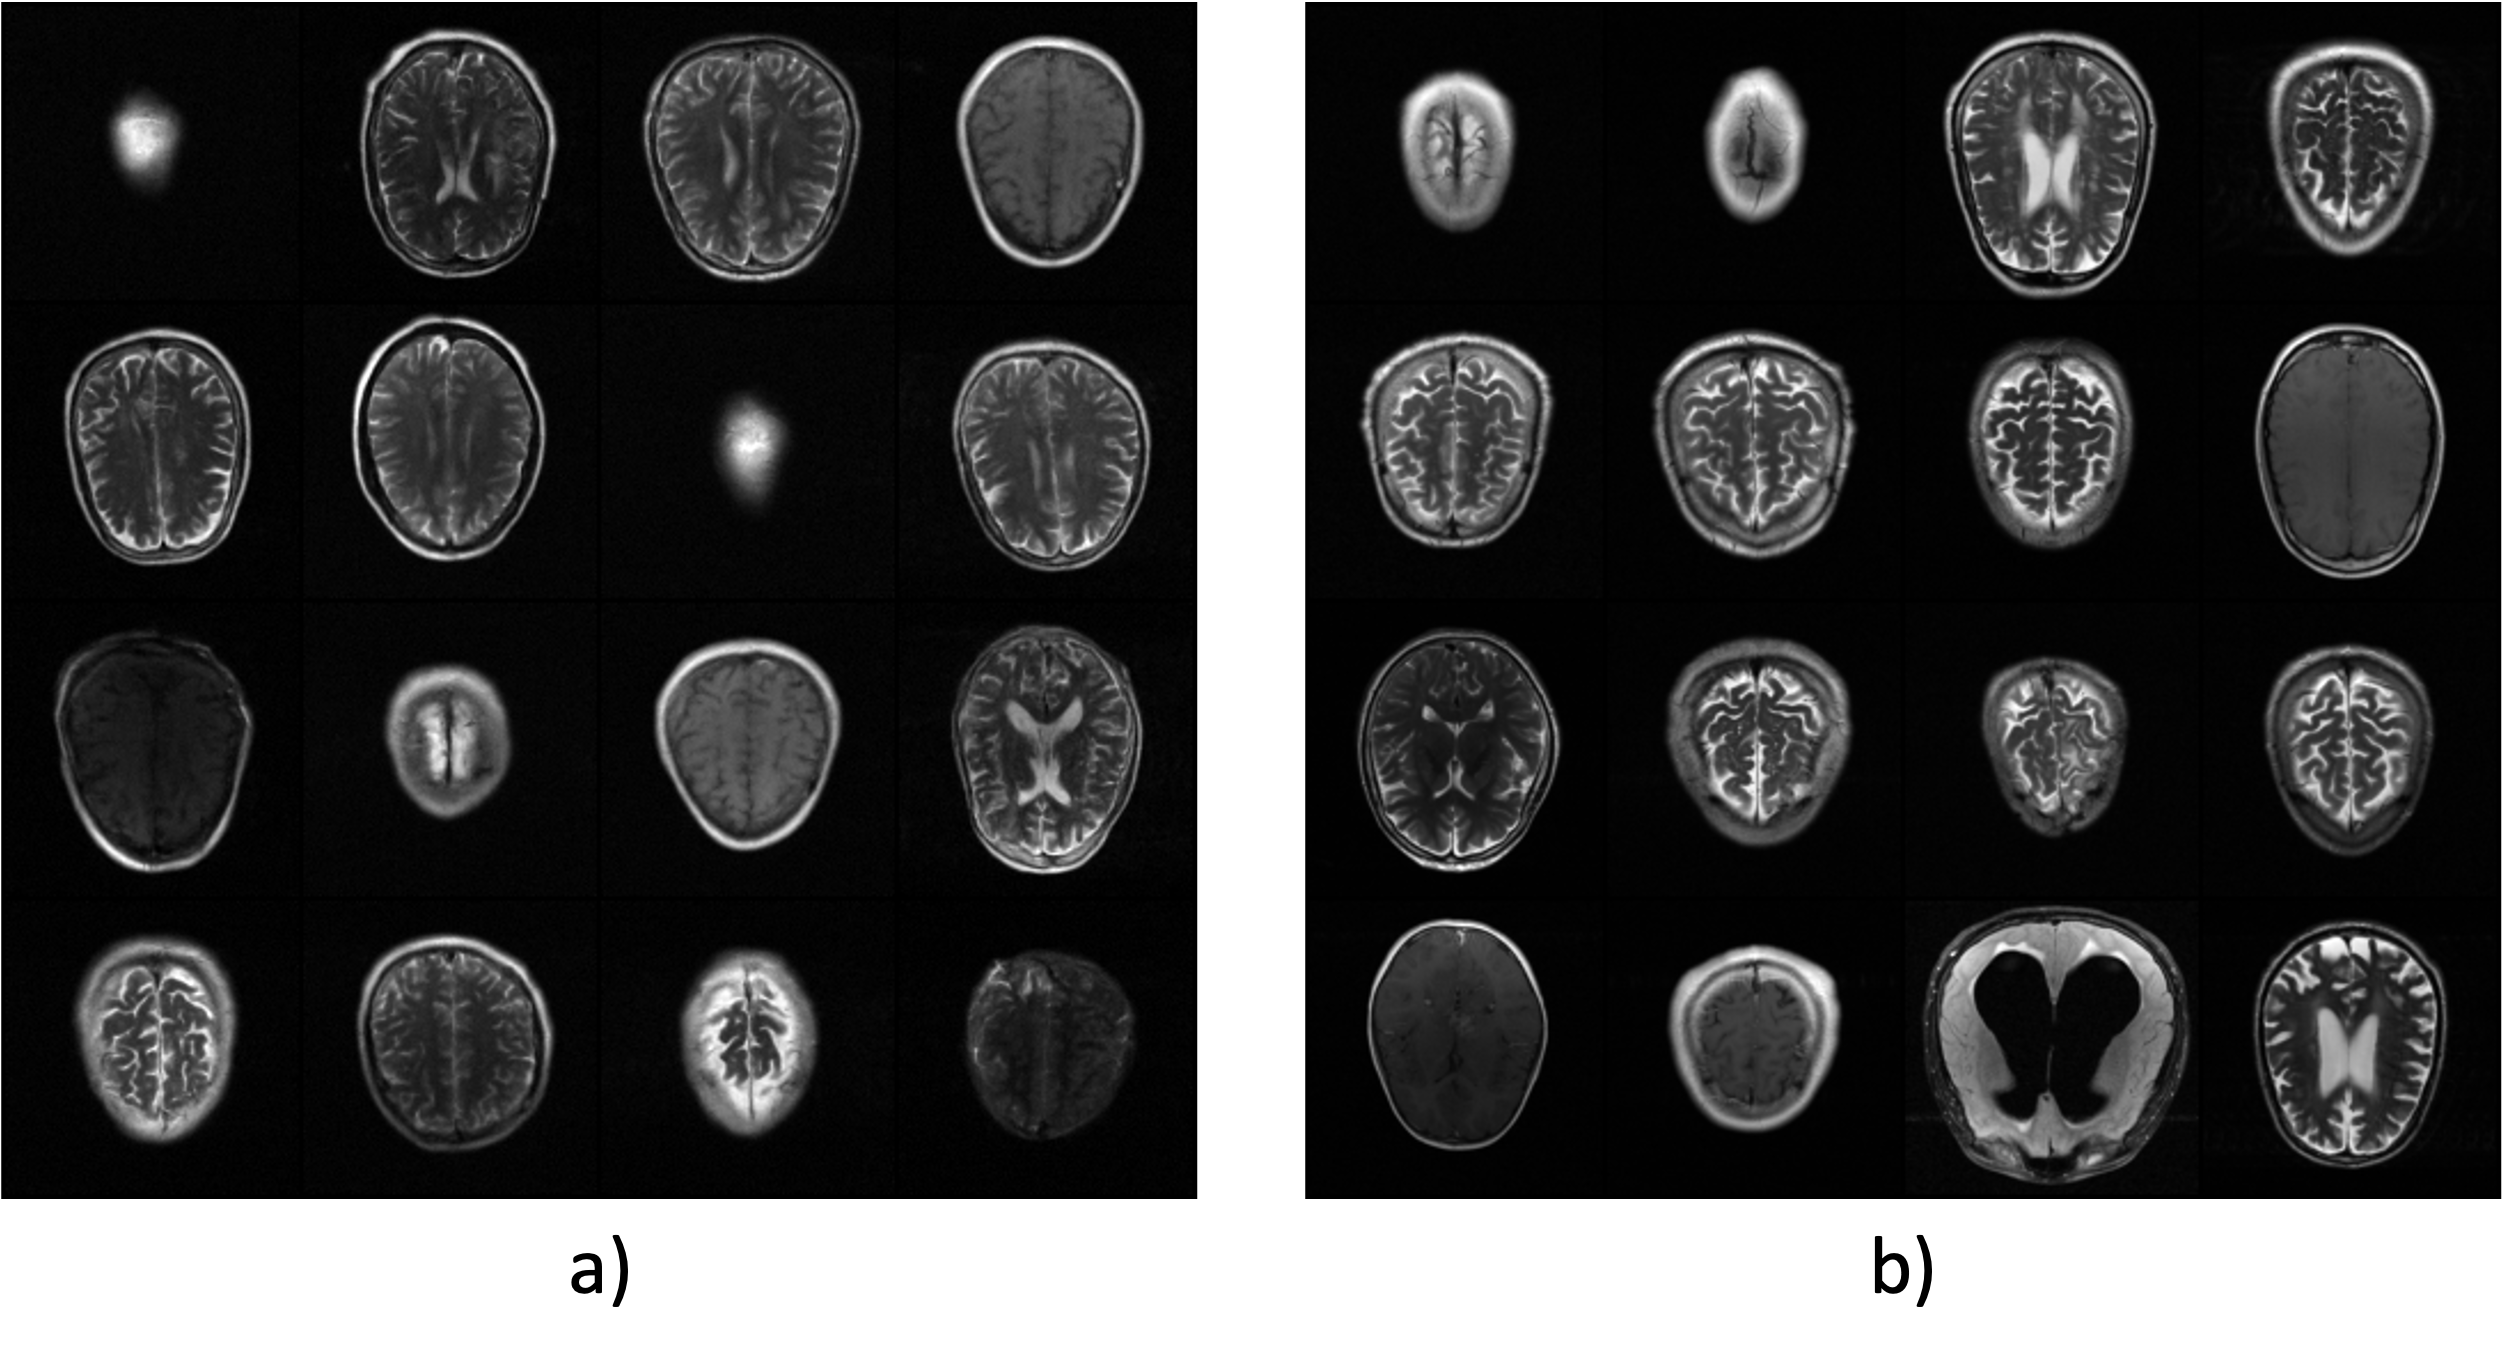
\includegraphics[width=.66\textwidth]{images/samples_unconditional.png}
    \caption[Samples from Data Set and Unconditional Sampling]{a) Unconditionally sampled examples, produced by the best-performing model; b) Examples from the training data set (fastMRI, RSS reconstruction); As can be seen, sample quality is comparable to the quality of the training samples and the variability among the samples is high, indicating a decent log-likelihood and mode coverage of the model.}
    \label{fig:uncondsampling}
\end{figure}

\section{Influence of Schedules and Image Size on the Forward Diffusion}
\label{sec:forward_diff_experiments}
Ho et al. had derived a closed form solution to the forward process of DDPMs and Nichol et al. investigated alternative options for the noise scheduling.~\autocite{ho2020denoising,nichol2021improved} They concluded that the important parameters to model are not the variances $\beta$ of the transitions, but the variances $1-\bar{\alpha}$ of the closed-form forward process, since they are the ones responsible for the destruction of information.

They decided to go with a squared cosine function, since this would be close to linear smooth out towards the critical beginning and end points of the process. In Fig.\ref{fig:alphadash} you can see how $1-\bar{\alpha}$ and $\beta$ behave for both approaches. It is immediately visible that the variances reach the maximum too early and flatten out for the linear schedule. This leads to the intuition that the last few steps are not very useful.

\begin{figure}[h]
    \centering
    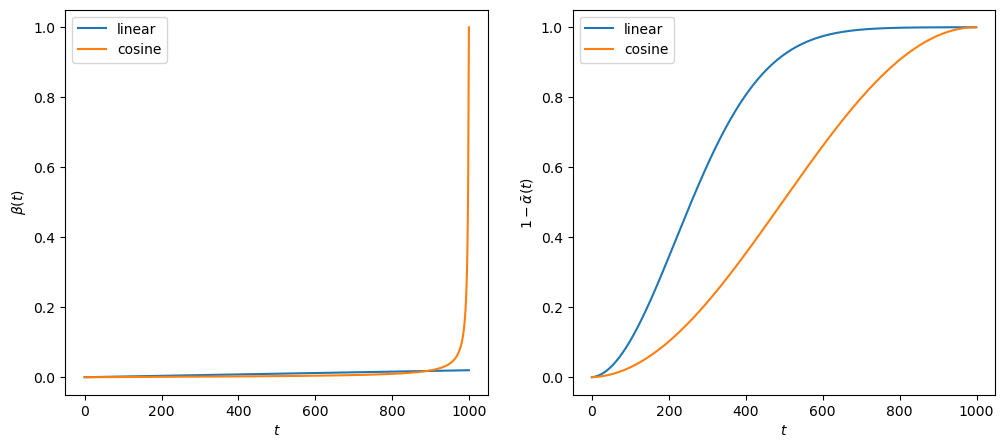
\includegraphics[width=.5\textwidth]{images/variance_schedule_alphadash.png}
    \caption{Variance Schedule Approaches: Modeling the $1-\bar{\alpha}$ as an approximate linear function (right cosine) and deriving $\beta$ (left cosine), or modeling $\beta$ as a linear function (left linear) and deriving $1-\bar{\alpha}$.}
    \label{fig:alphadash}
\end{figure}

The intution can experimentally confirmed by measuring how closely we get to isotropic noise when passing samples through the forward process. For this a batch of 50 times the same image was passed through the different steps of the process and the covariance matrix was calculated. As a metric for how close the covariance matrix was to the identity covariance matrix of pure i.i.d Gaussian noise, the identity matrix was subtracted and the mean of the absolute value of the matrix calculated. The results can be seen in Fig.~\ref{fig:noisecloseness} and confirm the intuition: When using linear scheduling we reach the closest point to pure noise already after around 600 steps for small images, and after around 700 for larger images. Cosine scheduling also performs worse on smaller images than on larger ones, but is still capable providing value for at least 850 timesteps.

\begin{figure}[h]
    \centering
    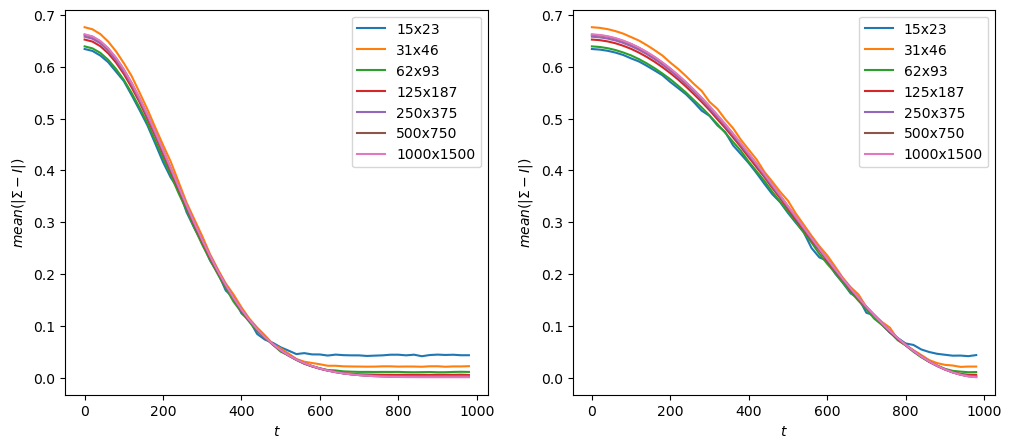
\includegraphics[width=.5\textwidth]{images/frobenius_norm.png}
    \caption{Closeness to noise for linear scheduling (left) and cosine scheduling (right).}
    \label{fig:noisecloseness}
\end{figure}

\section{Image Inpainting}
The work by Lugmayr et al.~\autocite{lugmayr2022repaint} was the main motivation to
\begin{figure}[h]
    \centering
    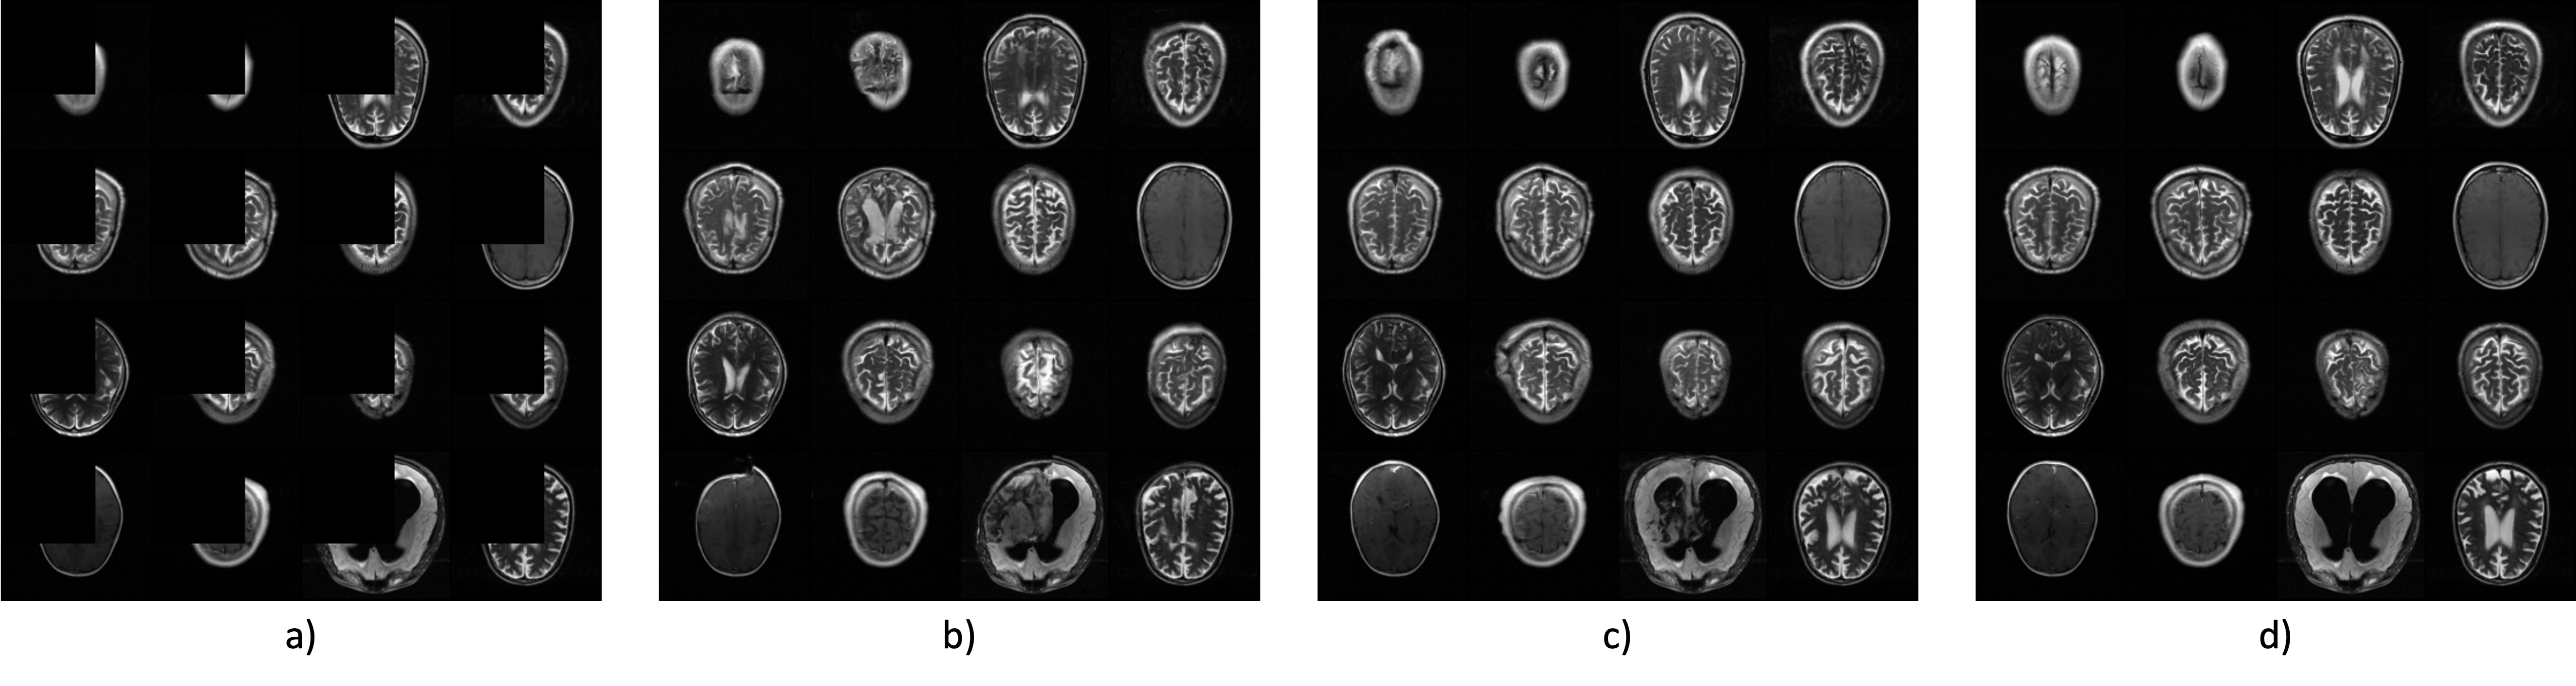
\includegraphics[width=.8\textwidth]{images/repaint.png}
    \caption[Inpainting and Resampling]{Inpainting and Resampling: a) Masked images used for the RePaint-style conditioning of the unconditional DDPM. b) Results from direct sampling. The reconstructed areas are often semantically wrong. c) Results from sampling with resampling. As observed by Lugmayr et al., the resampling strategy helps with semantically meaningful reconstruction. d) Ground truth images for comparison.}
\end{figure}

\section{Masked K-Space Substitution}
Lugmayr et al. use unconditional DDPMs to perform inpainting, which is a similar task to the reconstruction of undersampled MRI and are particularly successful by using resampling. This resampling process gives the network more time to create a globally semantically meaningful image.~\autocite{lugmayr2022repaint} Choi et al. replace low frequencies of the prediction with low frequencies of the latent representation of a target image to condition the diffusion process.~\autocite{choi2021ilvr} Since undersampled MRI still always contains global information, it was not expected, that resampling would have the same effect as with Lugmayr et al. Nevertheless it was expected to be an option for better sample fidelity through additional computation cost. The implementation follows below equation, where both, the latent prediction $x_t$ and the latent target $s_t$, are Fourier-transformed and predicted frequencies are replaced with known ones by the masking operation $\mathcal{M}$, wherever the information is available.
\begin{equation}
    x_{t-1} = x_t - \mathcal{F}^{-1}\left(\mathcal{M}\circ\mathcal{F}(x_t) + \mathcal{M}\circ\mathcal{F}(s_t)\right)
\end{equation}


\section{Variance in Predictions and Filtered Diffusion}
\label{sec:predvariance}
Aliasing arises from mismatches between predicted and introduced frequency information. Aliasing can be avoided by using low-pass filters, but the k-space mask is specifically sampled such that it also contains some information from higher frequencies. Naive low-pass filtering would make this information inaccessible and the sampling of those frequencies useless. Since the SNR (signal-to-noise-ratio) in natural images is much higher in the lower frequencies than in the lower ones, it was hypothesized that it might be possible to add frequency information gradually during the denoising process in order to avoid aliasing, lower frequencies first and higher ones only towards the end.

In order to empirically study this hypothesis, a single sample was denoised and its latent representations at every 10th timestep were saved. These latent representations were copied into batches of 100 equal latent representations and the denoising process was continued for all these batches. Fig.~\ref{fig:predvariance} shows 4 of these samples for a subset of starting points. As can be seen, when starting from $t\geq700$, the samples still have a lot of variability and share very few features. When starting later in the process, the samples look already very similar and only differ in some details. Since high frequencies are responsible for carrying information on details, this supports the hypothesis, but it becomes more evident, when looking at the variances of the spectral representations as seen in Fig.~\ref{fig:spectralvariance}. The variances were estimated over the frequency representations of all the final predictions in a batch (100 samples, denoised from $t$) and high variance means that this frequency was not yet determined at that specific $t$. As can be clearly seen in the figure, the variance is concentrated in the low frequencies when starting at larget $t$, and the variance in the low frequencies increases as the starting $t$ decreases. This again supports the hypothesis that high frequencies matter much more towards the end and that it might be possible to only introduce them later in the process.
\begin{figure}[h]
    \centering
    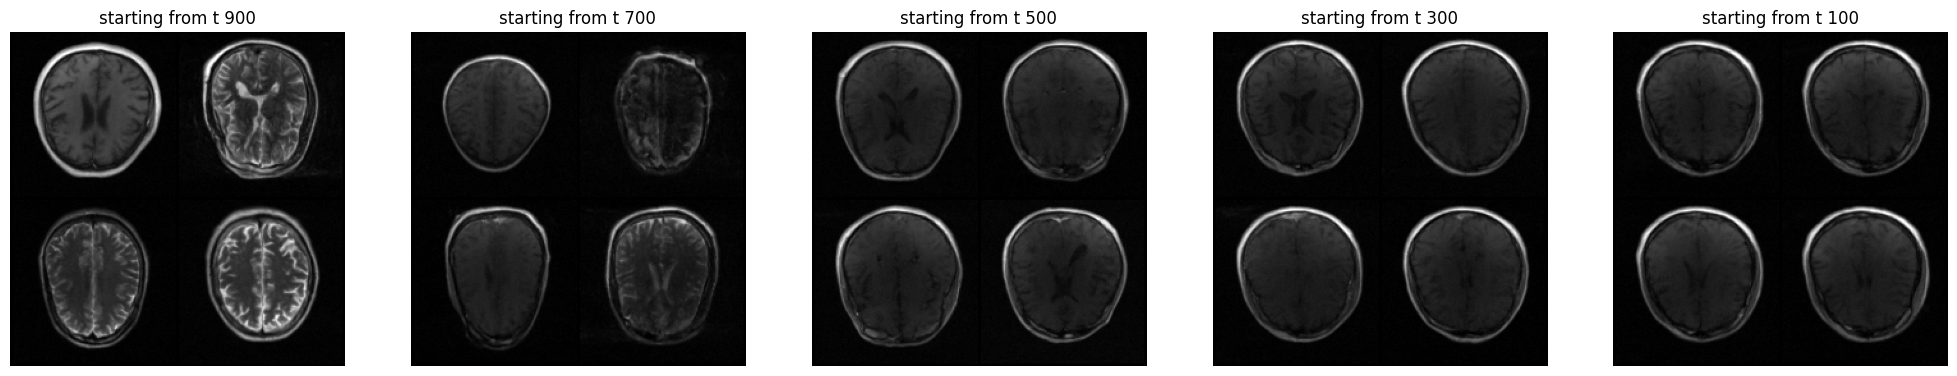
\includegraphics[width=.75\textwidth]{images/fixedlatents_variance.png}
    \caption[Variance in Predictions from Fixed Latents]{Variance in Predictions from Fixed Latents: The general shape of the final samples is already determined at $t=500$ and from there, the variability in the outputs is mostly about details of the structure.}
    \label{fig:predvariance}
\end{figure}

\begin{figure}[h]
    \centering
    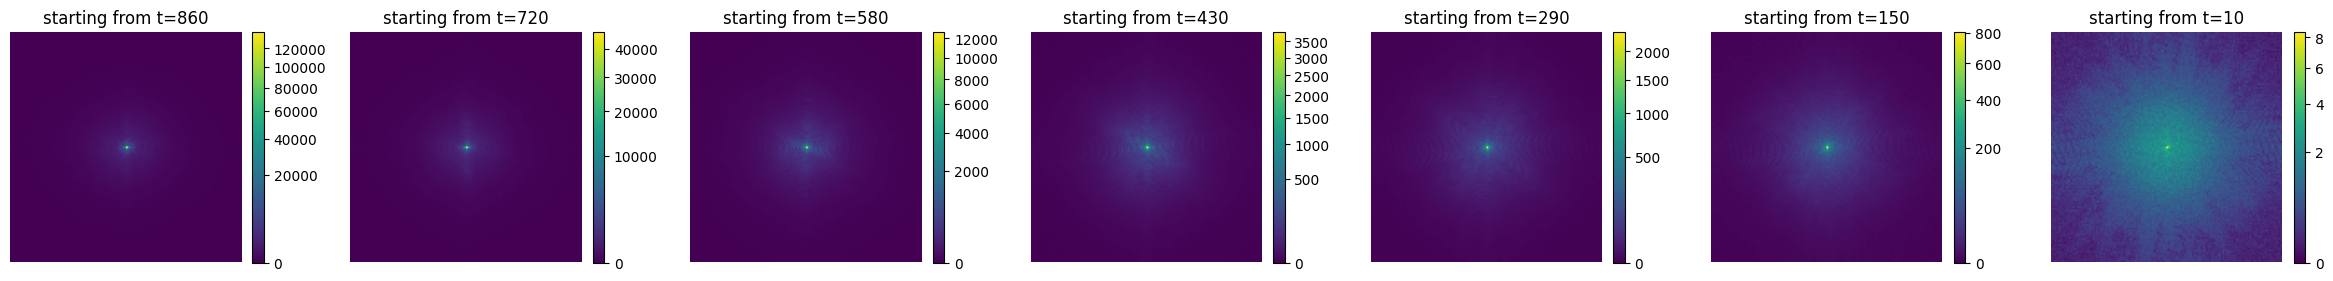
\includegraphics[width=\textwidth]{images/fixedlatents_varSpectra.png}
    \caption[Spectral Variance from Fixed Latents]{Variance in the Spectra when starting from Fixed Latents: When generating samples from fixed latent representation early in the denoising process, the variance of the spatial frequencies is highly concentrated in the center (e.g. $t=860$), overpowering the variance in the low frequencies by several orders of magnitude. The differences are smaller when starting late in the process (e.g. $t=10$), suggesting that fine details are only reconstructed at the very end. This hypothesis is also supported by the fact that natural images have lower SNR in the higher frequencies, which means that Gaussian perturbation affects them more and they can't carry much information until most of the noise is removed.}
    \label{fig:spectralvariance}
\end{figure}
\section{Frequency Replacement vs. Loss Function Guidance}
Results from section~\ref{sec:predvariance} suggested that lower frequencies only matter towards the end of the denoising process and guided diffusion with a loss function provides an additional to look at this by inspecting the gradients. Since these gradients are very noisy, they were averaged over a batch of 1200 equal samples. The results have been can be seen in Fig~\ref{fig:lossgradients} of the appendix.

\begin{figure}[h]
    \centering
    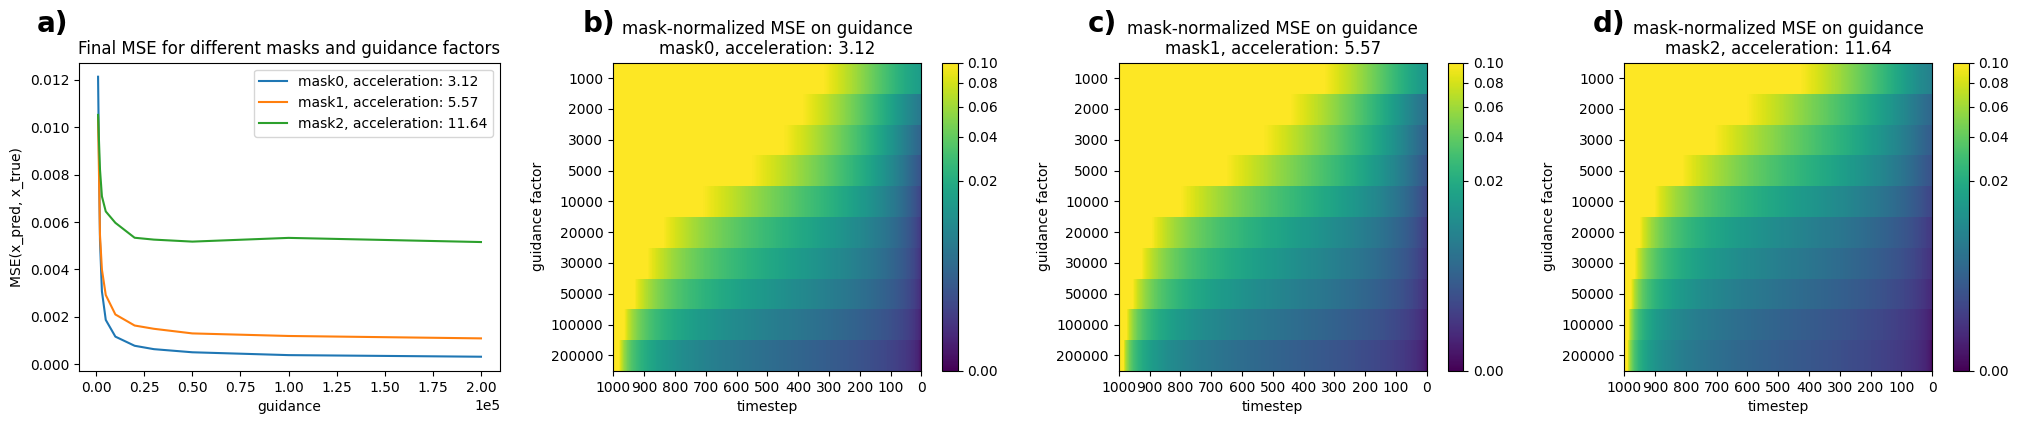
\includegraphics[width=\textwidth]{images/direct_sampling.png}
    \caption[Direct Sampling with Loss Guidance]{Results from Direct Sampling with Loss Guidance.}
\end{figure}
%% ----------------------------------------------------------------------------
% BIWI SA/MA thesis template
%
% Created 09/29/2006 by Andreas Ess
% Extended 13/02/2009 by Jan Lesniak - jlesniak@vision.ee.ethz.ch
%% ----------------------------------------------------------------------------
\newpage
\chapter{Discussion}
The discussion section gives an interpretation of what you have done \cite{day2006wap}:

\begin{itemize}
 \item \textit{What do your results mean?} Here you discuss, but you do not recapitulate results. Describe principles, relationships and generalizations shown. Also, mention inconsistencies or exceptions you found.
 \item \textit{How do your results relate to other's work?} Show how your work agrees or disagrees with other's work. Here you can rely on the information you presented in the ``related work'' section.
 \item \textit{What are implications and applications of your work?} State how your methods may be applied and what implications might be. 
\end{itemize}

\noindent Make sure that introduction/related work and the discussion section act as a pair, i.e. ``be sure the discussion section answers what the introduction section asked'' \cite{day2006wap}. 

%% ----------------------------------------------------------------------------
% BIWI SA/MA thesis template
%
% Created 09/29/2006 by Andreas Ess
% Extended 13/02/2009 by Jan Lesniak - jlesniak@vision.ee.ethz.ch
%% ----------------------------------------------------------------------------

\chapter{Conclusion}

List the conclusions of your work and give evidence for these. Often, the discussion and the conclusion sections are fused. 




%% ----------------------------------------------------------------------------
% If Appendix is needed
%% ----------------------------------------------------------------------------
\printbibliography[title=References]
\appendix
%% ----------------------------------------------------------------------------
% BIWI SA/MA thesis template
%
% Created 09/29/2006 by Andreas Ess
% Extended 13/02/2009 by Jan Lesniak - jlesniak@vision.ee.ethz.ch
%% ----------------------------------------------------------------------------
\chapter{Extended Derivations}
\section{Forward Process Marginal}
\label{app:forward}
Starting with transition distributions
\begin{equation}
    q(\bm{x}_t|\bm{x}_{t-1}) = \mathcal{N}(\sqrt{1-\beta_t} \bm{x}_{t-1}, \beta_t \bm{I})
\end{equation}
the reparameterization $\alpha = 1 - \beta$ is introduced
\begin{equation}
    q(\bm{x}_t|\bm{x}_{t-1}) = \mathcal{N}(\sqrt{\alpha_t} \bm{x}_{t-1}, (1-\alpha_t) \bm{I})
\end{equation}
which can be reformulated using the reparameterization trick as
\begin{align}
    \bm{x}_t & = \sqrt{\alpha_t}\bm{x}_{t-1} + \sqrt{1-\alpha_t}\cdot\mathcal{N}(\bm{0}, \bm{I}) \\
             & = \sqrt{\alpha_t}\bm{x}_{t-1} + \sqrt{1-\alpha_t} \cdot \bm{\epsilon}
\end{align}
with $\bm{\epsilon} \sim \mathcal{N}(\bm{0}, \bm{I})$. For the derivation it is helpful to use proper indices on the noise variables $\bm{\epsilon}_t$ and track them
\begin{equation}
    \bm{x}_{t} = \sqrt{\alpha_t}\bm{x}_{t-1} + \sqrt{1-\alpha_t}\bm{\epsilon_{t-1}}.
    \label{eq:forward_randomvar}
\end{equation}
The next term $\bm{x}_{t-1}$ can now be inserted into the formula by again using the reparameterization trick. Recalling that the sum $Z = X + Y$ of two normally distributed random variables $X \sim \mathcal{N}(\mu_X, \sigma_Y^2)$ and $Y \sim \mathcal{N}(\mu_Y, \sigma_Y^2)$ is again normally distributed according to $Z \sim \mathcal{N}(\mu_X + \mu_Y, \sigma_X^2 + \sigma_Y^2)$
\begin{align}
    x_t & = \sqrt{\alpha_t} \left( \sqrt{\alpha_{t-1}} \bm{x}_{t-2} + \sqrt{1-\alpha_{t-1}}\bm{\epsilon}_{t-2} \right) + \sqrt{1-\alpha_{t}} \bm{\epsilon}_{t-1} \\
        & = \sqrt{\alpha_{t}\alpha_{t-1}} \bm{x}_{t-2} + \sqrt{\alpha_{t}(1-\alpha_{t-1})} \bm{\epsilon}_{t-2} + \sqrt{1-\alpha_{t}} \bm{\epsilon}_{t-1}         \\
        & = \sqrt{\alpha_{t}\alpha_{t-1}} \bm{x}_{t-2} + \sqrt{\alpha_{t}(1-\alpha_{t-1}) + (1-\alpha_{t})} \bm{\bar{\epsilon}}_{t-2}
\end{align}
where $\bm{\bar{\epsilon}}_{t-2}$ is the noise variable for the sum of the random random variables up to $t-2$ (again $\bm{\bar{\epsilon}}_{t-2} \sim \mathcal{N}(\bm{0}, \bm{I})$). The second term can be simplified to
\begin{equation}
    \bm{x}_t = \sqrt{\alpha_{t}\alpha_{t-1}} \bm{x}_{t-2} + \sqrt{1-\alpha_t\alpha_{t-1}} \bm{\bar{\epsilon}}_{t-2}
\end{equation}
which is exactly the same form as in Eq.~\ref{eq:forward_randomvar}. The same procedure can be repeated in a recursive manner until the arrival at
\begin{equation}
    \bm{x}_t = \sqrt{\prod_{s=1}^{t}\alpha_s} \bm{x}_{0} + \sqrt{1-\prod_{s=1}^{t}\alpha_s} \bm{\bar{\epsilon}}_{0}.
\end{equation}
At this point we define $\bar{\alpha_t} = \prod_{s=1}^{t}\alpha_s$ and arrive at the final forms
\begin{align}
    \bm{x}_t                           & = \sqrt{\bar{\alpha}_{t}} \bm{x}_{0} + \sqrt{1-\bar{\alpha}_{t}} \bm{\bar{\epsilon}}_{0} \\
    \Rightarrow q(\bm{x}_t|\bm{x}_{0}) & = \mathcal{N}(\sqrt{\bar{\alpha}_t} \bm{x}_{0}, (1-\bar{\alpha}) \bm{I}).
\end{align}

\section{Derivation of Reverse Process Parameterization}
This derivation follows the work of Luo~\autocite{luo2022understanding} and starts with applying Bayes' rule to the forward process transition
\begin{equation}
    q(\bm{x}_t|\bm{x}_{t-1}, \bm{x}_0) = \frac{q(\bm{x}_{t-1}|\bm{x}_{t},\bm{x}_{0})q(\bm{x}_{t}|\bm{x}_{0})}{q(\bm{x}_{t-1}|\bm{x}_{0})}
\end{equation}
where $q(\bm{x}_t|\bm{x}_{t-1},\bm{x}_{0})$ is independent of $\bm{x}_0$ given $\bm{x}_{t-1}$ thanks to the factorization as a Markov chain and therefore
\begin{align}
    q(\bm{x}_t|\bm{x}_{t-1})                        & = \frac{q(\bm{x}_{t-1}|\bm{x}_{t},\bm{x}_0)q(\bm{x}_{t}|\bm{x}_{0})}{q(\bm{x}_{t-1}|\bm{x}_{0})}                                                                                                                                           \\
    \Rightarrow q(\bm{x}_{t-1}|\bm{x}_{t},\bm{x}_0) & = \frac{q(\bm{x}_t|\bm{x}_{t-1})q(\bm{x}_{t-1}|\bm{x}_{0})}{q(\bm{x}_t|\bm{x}_{0})}                                                                                                                                                        \\
                                                    & = \frac{\mathcal{N}(\sqrt{1-\beta_t}\bm{x_{t-1}}, \beta_t \bm{I}) \cdot \mathcal{N}(\sqrt{\bar{\alpha}_{t-1}}\bm{x_{t-1}}, (1-\bar{\alpha}_{t-1}) \bm{I})}{\mathcal{N}(\sqrt{\bar{\alpha}_{t}}\bm{x_{t-1}}, (1-\bar{\alpha}_{t}) \bm{I})}.
\end{align}
The means and variances can be inserted into the formula for the multivariate i.i.d Gaussian and after extended derivations (see~\autocite{luo2022understanding}, p.~12) one arrives at the final form
\begin{equation}
    q(\bm{x}_{t-1}|\bm{x}_{t},\bm{x}_0) \propto \mathcal{N}\left(\frac{\sqrt{\alpha_{t}}\left(1-\bar{\alpha}_{t-1}\right) \bm{x}_{t}+\sqrt{\bar{\alpha}_{t-1}}\left(1-\alpha_{t}\right) \bm{x}_{0}}{1-\bar{\alpha}_{t}}, \frac{\left(1-\alpha_{t}\right)\left(1-\bar{\alpha}_{t-1}\right)}{1-\bar{\alpha}_{t}} \mathbf{I}\right).
\end{equation}

\section{Derivation of ELBO/VLB}
In the case of a VAE we have
\begin{align}
    \log p_{\theta}(x) & = \log p_{\theta}(x) \int p_{\theta_{NN}}(z|x)dz                                                                                                                                                                           \\
                       & = \int \log p_{\theta}(x) p_{\theta_{NN}}(z|x)dz                                                                                                                                                                           \\
                       & = \mathbb{E}_{z\sim p_{\theta_{NN}}(z|x)}\left[\log p_{\theta}(x) \right]        \label{eq:A21}                                                                                                                            \\
                       & = \mathbb{E}_{z\sim p_{\theta_{NN}}(z|x)}\left[\log \frac{p_{\theta_{NN}}(x|z)p_{\theta_z}(z)}{p(z|x)}\right]   \label{eq:A31}                                                                                             \\
                       & = \mathbb{E}_{z\sim p_{\theta_{NN}}(z|x)}\left[\log \frac{p_{\theta_{NN}}(x|z)p_{\theta_z}(z)p_{\theta_{NN}}(z|x)}{p(z|x)p_{\theta_{NN}}(z|x)}\right]                      \label{eq:a35}                                  \\
                       & = \mathbb{E}_{z\sim p_{\theta_{NN}}(z|x)}\left[\log \frac{p_{\theta_{NN}}(x|z)p_{\theta_z}(z)}{p_{\theta_{NN}}(z|x)}\right] + \mathbb{E}_{z\sim p_{\theta_{NN}}(z|x)}\left[\log \frac{p_{\theta_{NN}}(z|x)}{p(z|x)}\right] \\
                       & = \mathbb{E}_{z\sim p_{\theta_{NN}}(z|x)}\left[\log \frac{p_{\theta_{NN}}(x|z)p_{\theta_z}(z)}{p_{\theta_{NN}}(z|x)}\right] + KL \left[p_{\theta_{NN}}(z|x)||p(z|x)\right].
\end{align}
Realize that only if $p_{\theta_{NN}}(z|x) = p(z|x)$ -- which is exactly when the the KL divergence is 0 -- we would get our original marginal log-likelihood $p_{\theta}(x)$ from the first term, as defined in Eq.~\ref{eq:A31}, by substituting and calculating back from Eq.~\ref{eq:a35}.
\begin{align}
    \mathbb{E}_{z\sim p_{\theta_{NN}}(z|x)}\left[\log \frac{p_{\theta_{NN}}(x|z)p_{\theta_z}(z)}{p_{\theta_{NN}}(z|x)}\right] & \stackrel{p_{\theta_{NN}}(z|x) = p(z|x)}{=} \mathbb{E}_{z\sim p_{\theta_{NN}}(z|x)}\underbrace{\left[\log \frac{p_{\theta_{NN}}(x|z)p_{\theta_z}(z)}{p(z|x)}\right]}_{p_{\theta}(x)} \\
                                                                                                                              & = \int \log p_{\theta}(x) p_{\theta_{NN}}(z|x) dz                                                                                                                                    \\
                                                                                                                              & = \log p_{\theta}(x)
\end{align}

\chapter{Training Metrics}
\begin{figure}
    \centering
    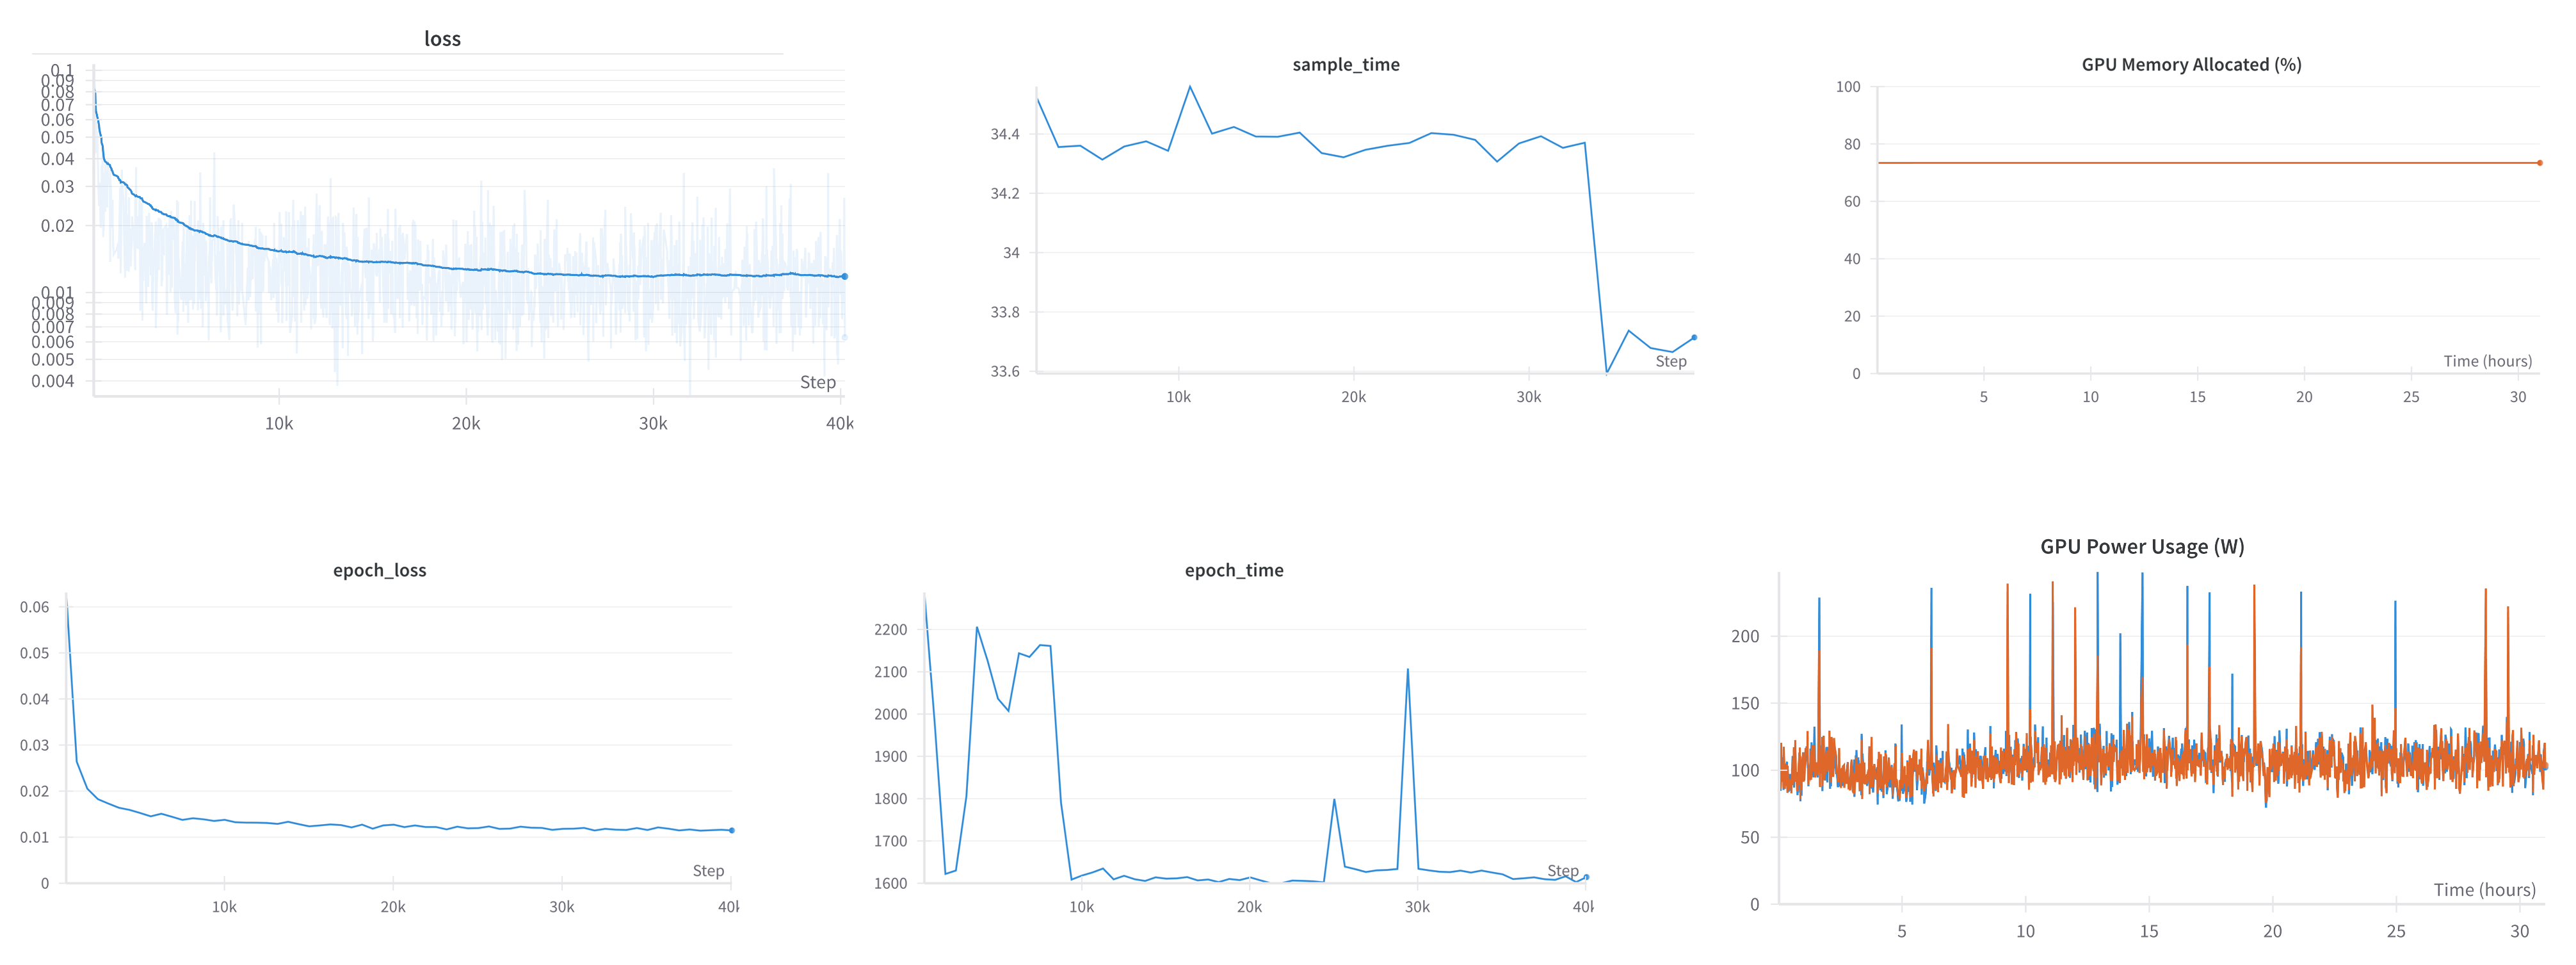
\includegraphics[width=\textwidth]{images/dutifulpondmetrics.png}
    \caption[Metrics from the Training Process of dutifulpond10]{Metrics from the Training Process of dutifulpond10}
    \label{fig:dutifulpond10}
\end{figure}

\begin{table}
    \centering
    \caption[Hyperparameter Overview dutifulpond10]{Overview over the Hyperparameters of dutifulpond10: The model was trained on all RSS reconstructions of the fastMRI brain dataset at a resolution of $128\times 128$, at a batch size of 48 and using the Adam optimizer at an initial learning rate of 0.0001.}
    \label{tab:dutifulpond10}
    \begin{tabular}{l l}
        Hyperparameter       & Value                             \\
        \hline
        dataset              & utils.datasets.FastMRIBrainTrain  \\
        dropout              & 0                                 \\
        backbone             & models.unet.UNet                  \\
        img\_size            & 128                               \\
        attention            & False                             \\
        loss\_func           & torch.nn.functional.mse\_loss     \\
        optimizer            & torch.optim.adam.Adam             \\
        activation           & torch.nn.modules.activation.SiLU  \\
        batch\_size          & 48                                \\
        in\_channels         & 1                                 \\
        kernel\_size         & 3                                 \\
        architecture         & models.diffusion.DiffusionModel   \\
        forward\_diff        & models.diffusion.ForwardDiffusion \\
        time\_enc\_dim       & 512                               \\
        learning\_rate       & 0.0001                            \\
        max\_timesteps       & 1000                              \\
        schedule\_type       & cosine                            \\
        from\_checkpoint     & False                             \\
        mixed\_precision     & True                              \\
        backbone\_enc\_depth & 5                                 \\
        unet\_init\_channels & 64                                \\
    \end{tabular}
\end{table}

\chapter{Samples \& Plots}
\begin{figure}
    \centering
    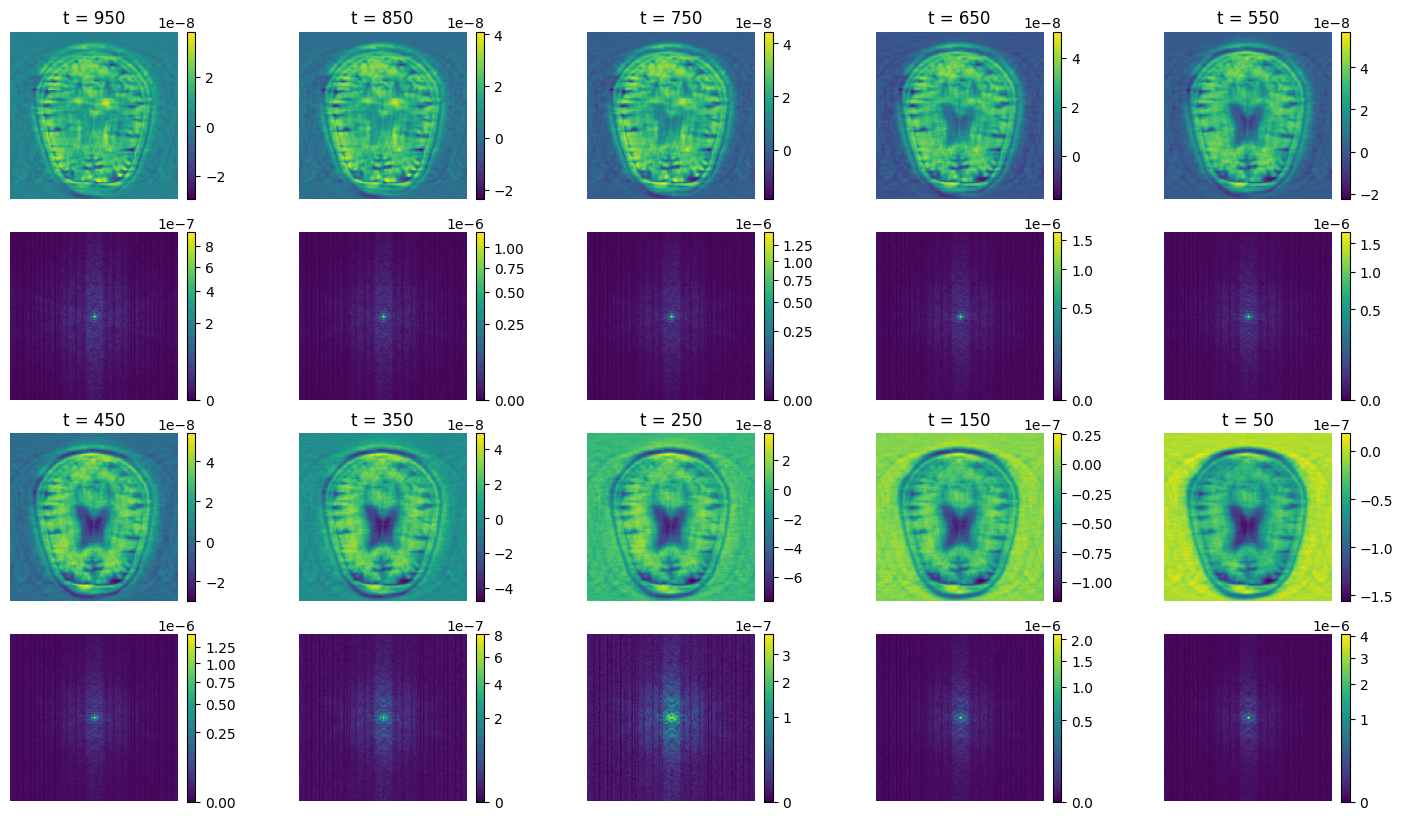
\includegraphics[width=.66\textwidth]{images/gradientspectra.png}
    \caption[Values and Spectra of Loss Gradients]{Values and Spectra of Loss Gradients: Middle and high frequencies seem to be particularly relevant around timestep $t=250$, which slightly counters the observations from section~\ref{sec:predvariance}.}
    \label{fig:lossgradients}
\end{figure}

\begin{figure}
    \centering
    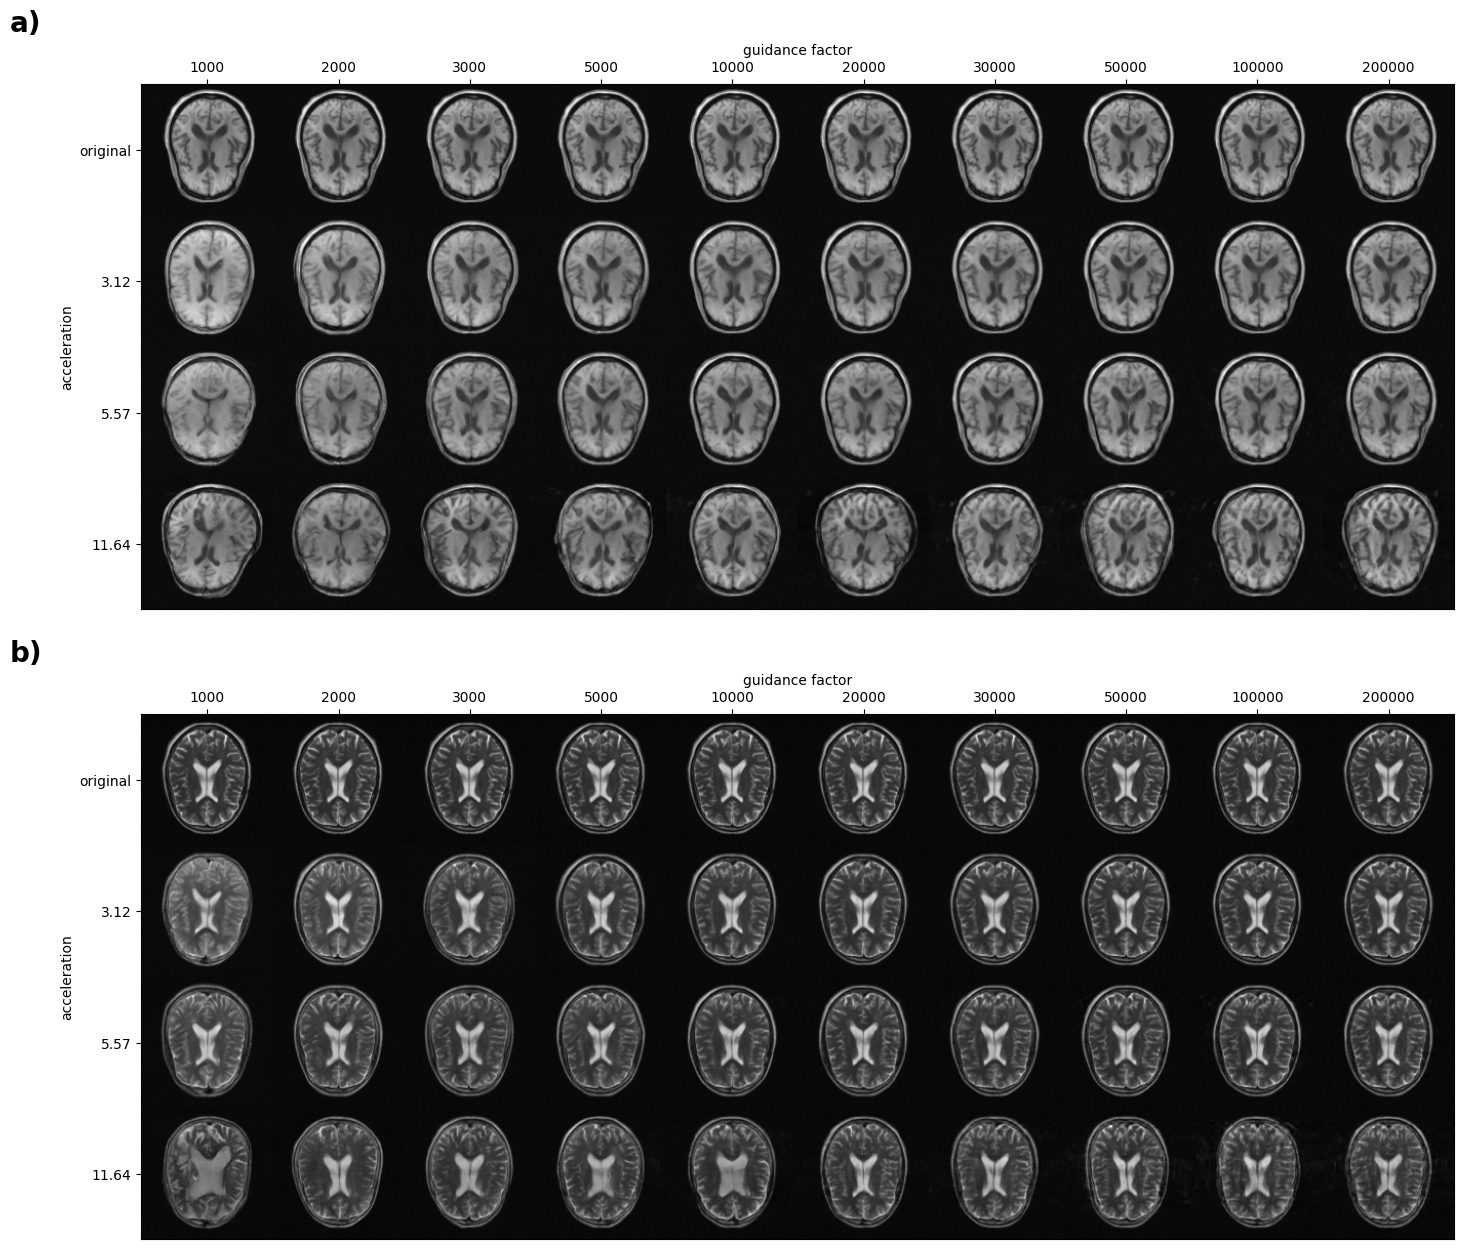
\includegraphics[width=\textwidth]{images/directsampling_comparison.png}
    \caption[Direct Sampling with Varying Masks and Guidance Factors]{Direct Sampling with Varying Masks and Guidance Factors: a) - b) Reconstructions of two samples, reconstructed using different masks (vertical) and different guidance factors (horizontal). For comparison, the top row is always the original samples. Low guidance factors lead to samples with less contrast and less adherence to the original, while high guidance factors combined with high accelerations can cause aliasing as observed in the lower right corner of a).}
    \label{fig:directsamplingcomparison}
\end{figure}

\begin{figure}
    \centering
    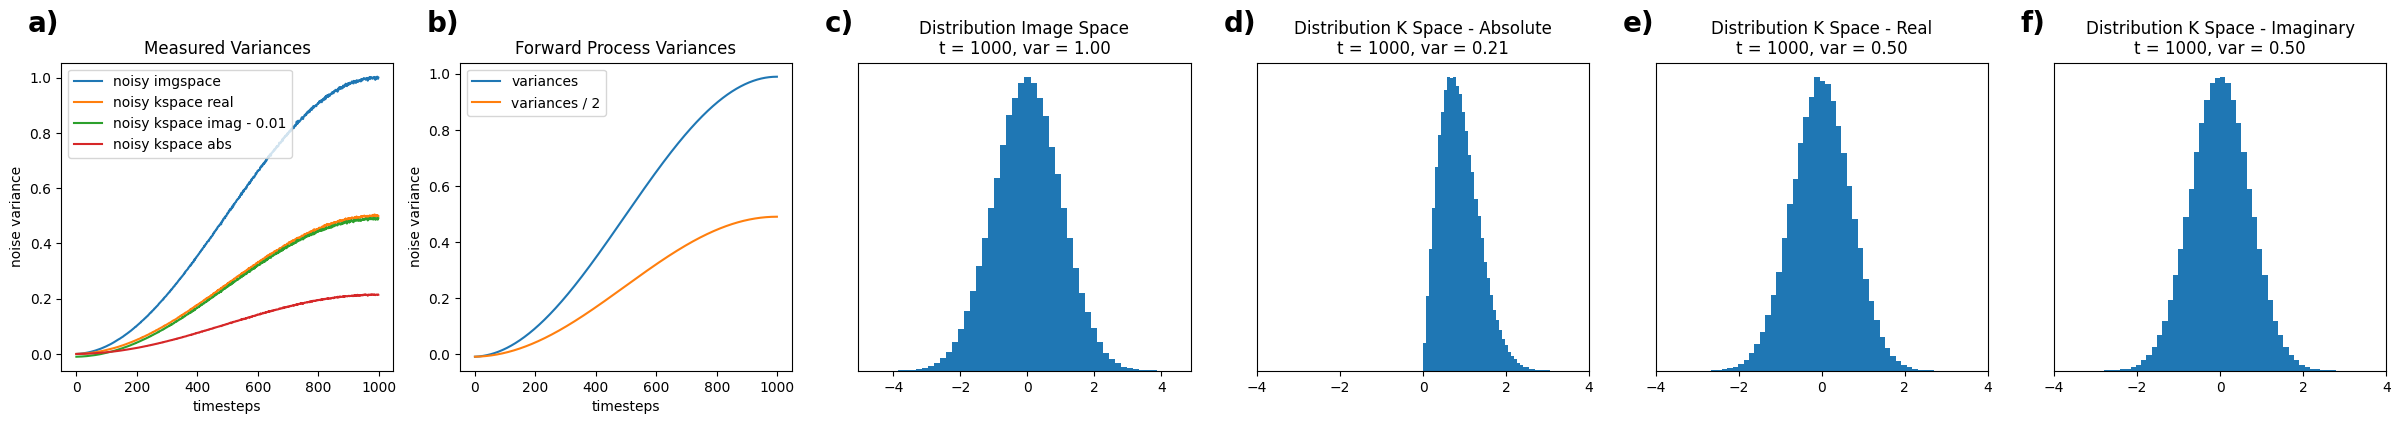
\includegraphics[width=\textwidth]{images/kspacedistribution.png}
    \caption[Noise Distribution of Latent K-Space]{Noise Distribution of Latent Space and Latent K-Space: a) Measured noise variances of forward process for image space as well as absolute, real and imaginary parts of k-space. The variances for the real and imaginary part are the same and were only shifted for visibility. They correspond to half the variances of the image space as can be seen in b) or when comparing the histograms in c), e) and f). The distribution of the absolute values of k-space in d) follows the Rice distribution.}
    \label{fig:kspacedistribution}
\end{figure}

\begin{figure}
    \centering
    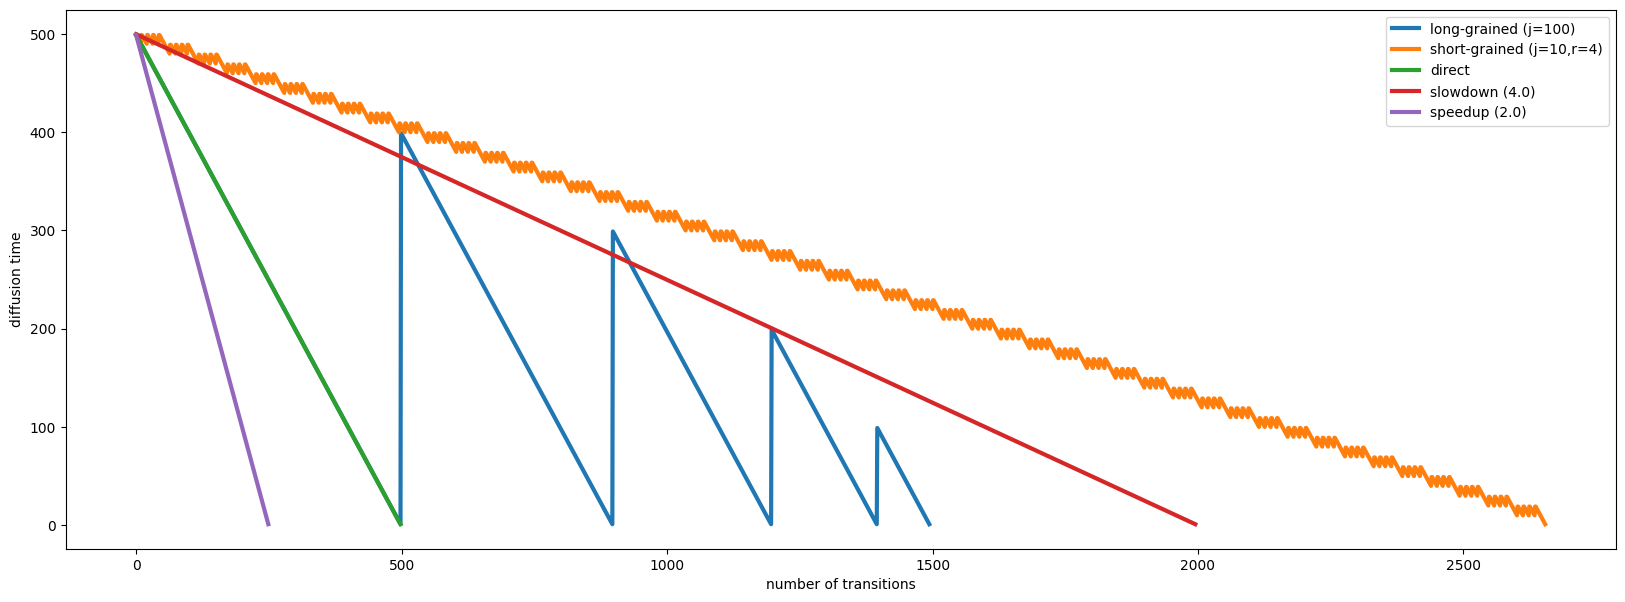
\includegraphics[width=\textwidth]{images/samplingstrategies.png}
    \caption[Sampling Strategies for DDPMs]{Sampling Strategies for DDPMs: This figure illustrates different strategies for trading off computation resources and sample quality. In order to make the details visible it is shown for a model with 500 timesteps, though the models in this work were trained on 1000 timesteps. Notable in the plot is the short-grained resampling, which is the resampling strategy used by Lugmayr et al~\autocite{lugmayr2022repaint} and they coined the terms \textit{jump length} ($j$) for the local region where resampling happens and \textit{resamplings} ($r$) for the number of resamplings in each localized area. Long-grained resampling repeats the sampling process over the last reverse diffusion timesteps, always shrinking it by $j$ timesteps with every iteration. The hope is that the latent representations at the start of a new resamplings are refined versions of the predictions from direct sampling at the corresponding timestep. By generalizing the time embedding, means and variances, it is further possible to make the model generalize to different numbers of timesteps, as illustrated with the slowdown and speedup.}
    \label{fig:stepsplot}
\end{figure}

\begin{figure}
    \centering
    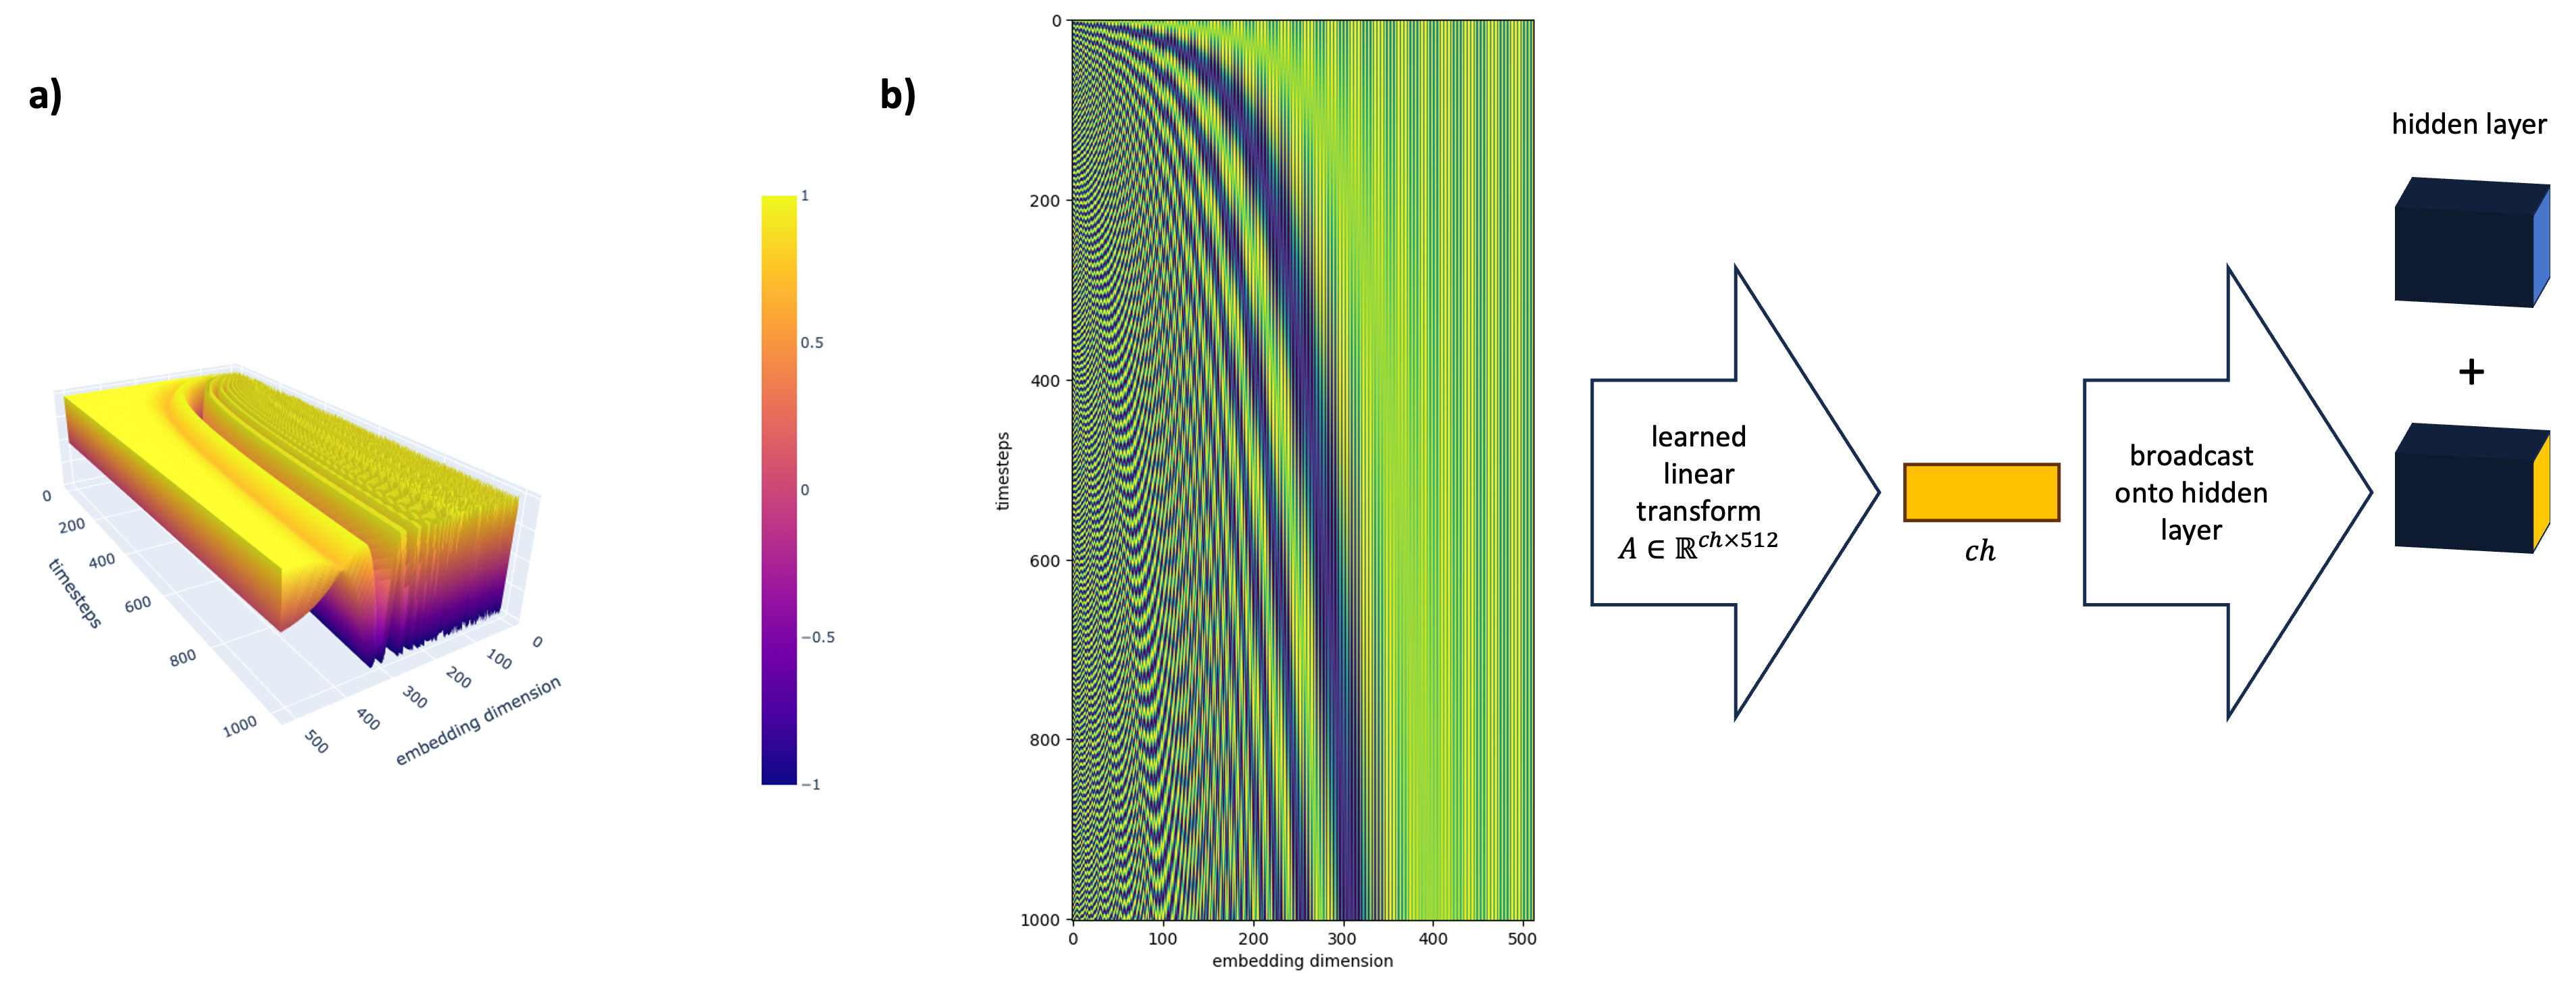
\includegraphics[width=\textwidth]{images/t_embedding.png}
    \caption[Plots of Time Encoding]{Time Encoding: a) The 3D surface plot of the time encodings shows that the low frequencies (encoded in the higher dimensions of the encoding) are responsible for differentiating between timesteps far apart, high frequencies for close timesteps. b) In order to condition the UNet on the time encodings, the encoding and decoding blocks include learned linear layers creating embeddings of the same dimension as the channels. The time embeddings are then added onto the hidden layer via a broadcasting operation.}
    \label{fig:timeencoding}
\end{figure}

%% ----------------------------------------------------------------------------
% Bibliography is stored in references.bib file, and can often be found
% online on webpages like dblp.uni-trier.de
%
% To include it in your thesis, run
%  pdflatex main
%  bibtex main
%  pdflatex main
%  pdflatex main
%
% This ensures all references are done correctly.
%% ----------------------------------------------------------------------------

\end{document}

